\documentclass[prd,showkeys,preprintnumbers,floatfix,superscriptaddress, nofootinbib]{revtex4}
\usepackage{float}
\usepackage{amsmath,amssymb}
\usepackage{graphicx}
\usepackage{mathtools,slashed}
\usepackage{bm}
\usepackage{comment}
\usepackage{color}
\usepackage{subfigure}
\usepackage{array}
\usepackage{multirow}
\usepackage{url}
\usepackage{color}
\usepackage[T1]{fontenc}
\usepackage[latin9]{inputenc}
\usepackage{graphicx}
\usepackage{esint}
\usepackage{hyperref}
\usepackage{atbegshi}
\usepackage{lipsum}
\newcommand{\nn}[0]{\nonumber} 
 \newcommand{\raul}[0]{ \color{blue} }
 \newcommand{\red}[0]{ \color{red} }
\newcommand{\W}[0]{{\mathcal{W}}}
\newcommand{\Wtildf}[0]{{\mathcal{W}}_{L,{\rm df}}}
\newcommand{\Wdf}[0]{{\mathcal{W}}_{\rm df}}
\newcommand{\RLL}[0]{\mathcal{R}}
\newcommand{\w}[0]{w}
\newcommand{\mh}[0]{\color{red} \bf }
\newcommand{\Epipi}{E_{\pi\pi}}




\begin{document}
 \preprint{\vbox{\hbox{JLAB-THY-??-???} }}
\title{Obtaining form factors of resonances and bound states from lattice QCD}

%%%%%%%%%%
\author{Alessandro Baroni}
%
\email[e-mail: ]{abaro008@odu.edu}
%
\affiliation{
Department of Physics and Astronomy University of South Carolina, \\ 
712 Main Street, Columbia, SC 29208, USA
}
%%%%%%%%%%

%%%%%%%%%%
\author{Ra\'ul A.~Brice\~no}
%
\email[e-mail: ]{rbriceno@jlab.org}
%
\affiliation{Thomas Jefferson National Accelerator Facility, 12000 Jefferson Avenue, Newport News, VA 23606, USA}
\affiliation{ Department of Physics, Old Dominion University, Norfolk, VA 23529, USA}
%%%%%%%%%%

%%%%%%%%%%
\author{Bipasha Chakraborty}
%
\email[e-mail: ]{bipasha@jlab.org}
%
\affiliation{
Thomas Jefferson National Accelerator Facility, 12000 Jefferson Avenue, Newport News, VA 23606, USA\\
}
%%%%%%%%%%





%%%%%%%%%%

\author{Maxwell T.~Hansen}
%
\email[e-mail: ]{hansen@kph.uni-mainz.de}
%
\affiliation{
Institut f\"ur Kernphysik and Helmholtz Institute Mainz, Johannes Gutenberg-Universit\"at Mainz,
55099 Mainz, Germany\\
}
%%%%%%%%%%
%%%%%%%%%%
\author{Felipe Ortega}
%
\email[e-mail: ]{felipeortegagama@gmail.com}
%
\affiliation{
?????//
}
%%%%%%%%%%

%%%%%%%%%%%%%%%%%%%%%%%%%%%%%%%%%%%%%%%%%%%%%%%%%%%%%%%%%%%%%%%%%%%%%%
\author{David~J.~Wilson}
\email[]{djwilson@maths.tcd.ie}
\affiliation{School of Mathematics, Trinity College, Dublin~2, Ireland}
%%%%%%%%%%%%%%%%%%%%%%%%%%%%%%%%%%%%%%%%%%%%%%%%%%%%%%%%%%%%%%%%%%%%%%



\date{\today}

\begin{abstract}
This {\em master document} details all steps in the HadSpec numerical lattice QCD calculation of the $\rho$ form factor. The novel aspect of this calculation is that the resonance nature of the $\rho$ is rigorously accomodated. This is achieved by first determining the infinite-volume matrix element $\langle \pi \pi, \text{out} \vert \mathcal J^\mu \vert \pi \pi, \text{in} \rangle$ and then analytically continuing both the initial and final two-pion state energies into the complex plane, to the $\rho$ pole.
 \end{abstract}

\keywords{finite volume, lattice QCD}

\nopagebreak
\maketitle

\tableofcontents

\clearpage
\section{To do list}
%\begin{table}
\begin{center}
  \begin{tabular}{ c | c | c | c | c | c | c  }
    \hline
                           & \ \ Alessandro \ \  & \ \  Ra\'ul \ \  & \ \ Bipasha \ \  & \ \  Max \ \  & \ \  Felipe \ \  & \ \  Dave \ \   \\ \hline \\[-10pt] \hline
%
{\bf Toy analyses} &                          &                      &                        &                   &                    &                      \\ \hline
{\em scalar}        &                            &                      &                        &                   &                     &                        \\ \hline
{\em vector}        &                            &                      &                        &                   &                     &                       \\ \hline \\[-10pt] \hline
%
 {\bf $\pi$ form factor}&                     &                      &                        &                   &                     &                      \\ \hline
 {\em subduction}  &                          & date              & date                &                   &                     &                      \\ \hline
 {\em subtask 2}  &                            &                      &                        &                   &                     &                      \\ \hline \\[-10pt] \hline
%
{\bf $\rho$ form factor} &                  &                      &                        &                   &                    &                      \\ \hline
{\em subduction}      &                      & date              & date                &                   &                     &                        \\ \hline
{\em subtask 2}        &                      &                      &                        &                   &                     &                       \\ \hline \\[-10pt] \hline  
%
{\bf LL code}       &                            &                      &                        &                   &                     &                      \\ \hline
{\em subtask 1}  &                            &                      &                        &                   &                     & date               \\ \hline \\[-10pt] \hline
%
{\bf Evaluate $G$}  &                        &                      &                        &                   &                     &                      \\ \hline
{\em accelerated form} & date          &                      &                        & date           & date            &                      \\ \hline  
%
\end{tabular}
\end{center}


\begin{center}
  \begin{tabular}{ c | c | c | c | c | c | c  }
    \hline
                           & \ \ Alessandro \ \  & \ \  Ra\'ul \ \  & \ \ Bipasha \ \  & \ \  Max \ \  & \ \  Felipe \ \  & \ \  Dave \ \   \\ \hline \\[-10pt] \hline
%
 {\bf General LQCD} &                      &                      &                        &                   &                     &                      \\ \hline
 {\em gen props} &                            & date              & date                & date           &                     &                      \\ \hline
 {\em contractions} &                         & date             & date                & date            &                     &                      \\ \hline  
%
\end{tabular}
\end{center}


\subsection{Toy analyses}

Perform a toy-model analysis of  the elastic form factor for a scalar system, i.e.~the $\sigma$. Here there is only a single form factor. Then repeat the analysis for a vector system, i.e.~the $\rho$. Here there are three form factors. In the case of the vector things are more complicated, not just because of the finite-volume effects, but also the Lorentz decomposition. Specifically we can no long disentangle the three form-factors independently because different irreps have different energies and virtualities.

\subsection{General LQCD}

\subsection{$\pi$ form factor}

\subsection{$\rho$ form factor}

\subsection{LL code}

\subsection{Evaluate $G$}
%\end{table}

 %%%%%%%%%%%%%%%%%%%%%%%%%%%%%%%%%%%%%%%%%%
%\section{Introduction}
%{\raul we need to do a fake data analysis. It would be good to have some models for the $\pi\pi\gamma^\star\to\pi\pi$ amplitudes. We should do the analysis when there is a single form factor, namely for a scalar channel (like the $\sigma$), and when there are three form factor, namely for the vector channel. }

\clearpage
\section{Form factors, amplitudes, and Lorentz decomposition}
Before describing how the desired observables can be extracted using lattice QCD, it is instructive to discuss the infinite-volume quantities that we aim to calculate. Our aim is two-fold:
	\begin{enumerate}
	\item Explain how different components of the $\pi\pi\gamma^\star\to\pi\pi$ amplitude can be extracted from lattice QCD. We will focus on the components where both the initial and final state have been projected onto an isotriplet. 
	\item Constrain the amplitude as much as possible, in the largest possible kinematic window. We can then analytically continue initial and final states to the $\rho$ pole to obtain the four form factors of the $\rho$. 
	\end{enumerate}

	In order to take the first step, we will need the formalism introduced in Ref.~\cite{Briceno:2015tza}. The approach is sketched in Fig.~\ref{fig:flowchart} and is reviewed in detail in Sec.~\ref{sec:pipigs_pipi}. The two key inputs, in addition to the standard matrix elements, are 
	\begin{itemize}
	\item the $\pi\pi\to\pi\pi$ scattering amplitude,
	\item the single pion form factor, $\langle \pi \vert \mathcal J^\mu \vert \pi \rangle$.
	\end{itemize}
	
	In this section we begin by reviewing basic consequences of the symmetries of the infinite-volume system: isospin, parity, G-parity, angular momentum, and charge conservation. 
	
 %%%%%%%%%%%%%%%%%%%%%%%%%%%%%%%%%%%%%%%%%%%
\begin{figure*}[t]
\begin{center}
\subfigure[]{
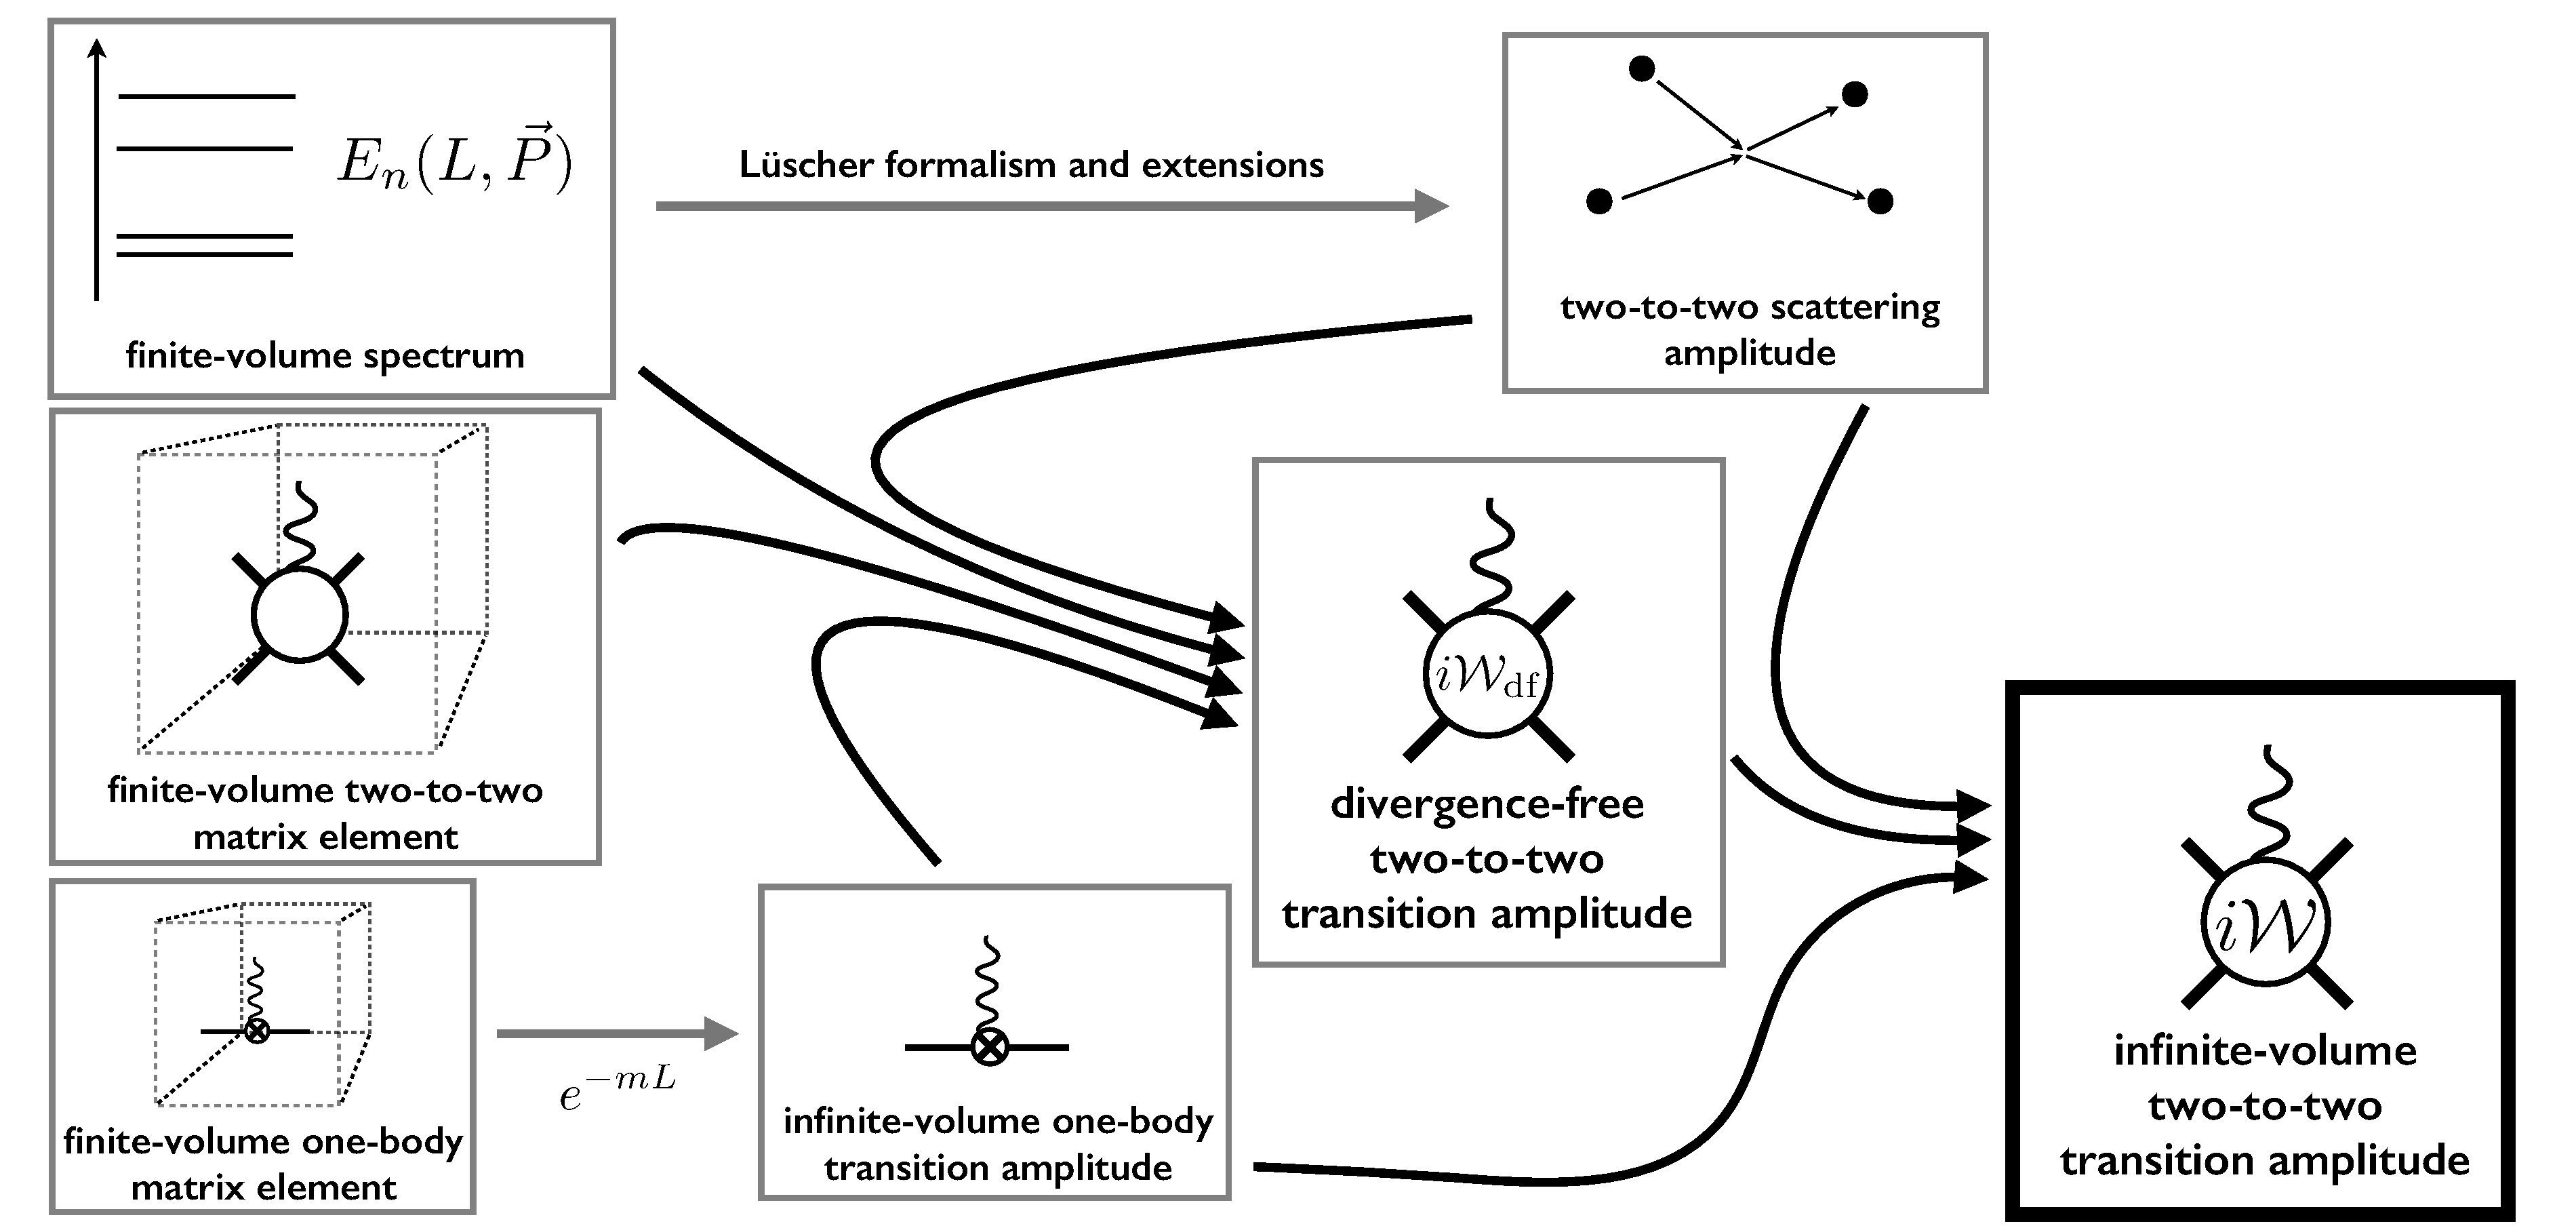
\includegraphics[width=.8\textwidth]{figs/flowchart2}}
\caption{Flowchart summarizing the process for extracting resonance form factors using the formalsim of Ref.~\cite{Briceno:2015tza}. {\mh [check update]}}\label{fig:flowchart}
\end{center}
\end{figure*}
 %%%%%%%%%%%%%%%%%%%%%%%%%%%%%%%%%%%%%%%%%%%

 %%%%%%%%%%%%%%%%%%%%%%%%%%%%%%%%%%%%%%%%%%
\subsection{Isospin and charge}

The aim of this project is to explain how one can obtain the form factors of a resonance. In particular, we will be focusing on electromagnetic form factors and to resonances that couple to $\pi\pi$ states. With this in mind, it is useful to review the isospin projections of the $\pi\pi$ system, and the resonance content of each channel, beginning with the isostensor. This channel has no resonances; the individual states are given by
\begin{align}
|I=2,m_I=2\rangle&=|\pi^+\pi^+\rangle \,,\\
|I=2,m_I=1\rangle&=\frac{1}{\sqrt{2}}\left(|\pi^+\pi^0\rangle+|\pi^0\pi^+\rangle\right) \,,\\
|I=2,m_I=0\rangle&=\frac{1}{\sqrt{6}}\left(|\pi^+\pi^-\rangle+|\pi^-\pi^+\rangle+2|\pi^0\pi^0\rangle\right) \,.
\end{align}

By contrast, the isovector channel contains the rho resonance, $\rho=(\rho^+,\rho^0,\rho^-)$. The $\rho^0$ is neutral and an eigenstate of charge conjugation. Furthermore, the electromagnetic current is odd under charge conjugation, $C\bar{\psi}\gamma^\mu \psi C=-\bar{\psi}\gamma^\mu \psi$. This implies 
\begin{align}
\langle \rho^0|\bar{\psi}\gamma^\mu \psi | \rho^0\rangle
=
\langle \rho^0|C(C\bar{\psi}\gamma^\mu \psi C)C| \rho^0\rangle
=
-\langle \rho^0|\bar{\psi}\gamma^\mu \psi | \rho^0\rangle=0.
\end{align}
Similarly, one concludes that the electromagnetic matrix elements of the $\pi^0$ vanishes. Note, since the $\rho^0$ is negative under charge conjugation and the $\pi^0$ is even, the $\langle \rho^0|\bar{\psi}\gamma^\mu \psi | \pi^0\rangle$ matrix element need not be zero, similarly the $\pi^0\to\gamma\gamma$ is not zero.

 Since the $\rho^0$ form factors are zero, we will focus on the $\rho^+$. The definition of $I=1$ $\pi\pi$ states and the association to the $\rho$ states is as follows:
\begin{align}
\rho^+:\hspace{.5cm}|I=1,m_I=1\rangle&=\frac{1}{\sqrt{2}}\left(|\pi^+\pi^0\rangle-|\pi^0\pi^+\rangle\right),\\
\rho^0:\hspace{.5cm}|I=1,m_I=0\rangle&=\frac{1}{\sqrt{2}}\left(|\pi^+\pi^-\rangle-|\pi^-\pi^+\rangle\right) \,.
\end{align}
Here we notice two things. As already stated above, we will need the form factors of the individual pions to calculate the rho form factor. Given that only that of the $\pi^+$ is nonzero, we will only need to calculate this one. 
 

Finally, the isoscalar channel couples to the $\sigma$,
\begin{align}
\sigma:\hspace{.5cm}|I=0,m_I=0\rangle&=\frac{1}{\sqrt{3}}\left(|\pi^+\pi^-\rangle+|\pi^-\pi^+\rangle-|\pi^0\pi^0\rangle\right).
\end{align}
This, of course, is neutral and is even under charge conjugation. As a result, similarly for the $\rho^0$ and $\pi^0$ its electromagnetic form factor vanishes. 

In conclusion, of the $\pi\pi$ channels, the one that is most sensible to consider here is $(I,m_I)=(1,1)$, since this is the only one that could have a resonance form factors. The $\rho^+$ is a vector, implying that it has three-independent form factors to determine, the charge, magnetic and quadrupole form factors. These are proportional to the the charge, magnetic moment, and quadrupole moment of the $\rho^+$. Furthermore, one can obtain the correspond radii of the $\rho^+$. As we argue below, in practice this \emph{might} require to calculate four independent amplitudes from lattice QCD calculations. As one analytically continues these onto the $\rho$ pole, one of them will vanish, resulting in three non-zero form factors. 


After examining which matrix elements are allowed in the following subsection, we discuss the Lorentz decomposition of the matrix elements in terms of form factors in Sec.~\ref{sec:Lorentz_FFs}.

 %%%%%%%%%%%%%%%%%%%%%%%%%%%%%%%%%%%%%%%%%%%%%%
 \subsection{Allowed matrix elements}

We are interested in evaluating matrix elements of the QED current
\begin{align}
{\mathcal{J}}^{\mu}=q_u\bar{u}\gamma^\mu u+q_d\bar{d}\gamma^\mu d= \big (2\bar{u}\gamma^\mu u-\bar{d}\gamma^\mu d \big )/3 \,.
\end{align} 
It is convenient to decompose this into an isovector and isoscalar current, 
\begin{align}
{\mathcal{J}}^{\mu}&=\frac{ \rho^{0,\mu}}{\sqrt{2}}+\frac{\omega^{\mu}}{3\sqrt{2}} \,,
\end{align}
where
\begin{align}
\rho^{0,\mu}&= \big ( \bar{u}\gamma^\mu u-\bar{d}\gamma^\mu d \big )/\sqrt{2} \,,\\
\omega^{\mu}&= \big (\bar{u}\gamma^\mu u+\bar{d}\gamma^\mu d \big )/\sqrt{2} \,.
\end{align} 
The $\rho^{0,\mu}$ component has the quantum number of the $I_z=0$ component of the $\rho$ meson, namely $I^G(J^{P})=1^{+}(1^{-})$,%
%FOOTNOTE
\footnote{$I=$isospin, $G=$G-parity, $J$=total angular momentum, $P$=parity.}
while the $\omega^{\mu}$ piece has the quantum numbers of the $\omega$ meson, $0^{-}(1^{-})$. Strictly speaking, these are the quantum numbers of the spatial piece of the current; the temporal components are related via Lorentz symmetry. 


For the single-pion matrix elements, one can explicitly evaluate the contractions {\raul (I get that the disconnected piece of the $\rho^{0,\mu}$ current vanishes, but not for the $\omega$ piece, so not $100\%$ sure about this)}, to find that only the component of the QED current that survives the $\rho$\,-like piece. {\mh [I am not so sure if it is true that we can see the vanishing by evaluating contractions. Consider in particular
\begin{align}
\langle \pi  \vert \omega^\mu \vert \pi \rangle & \propto \langle 0 \vert ( \bar q \tau^a \gamma_5 q )   (\bar{q} \mathbb I \gamma^\mu  q)  ( \overline q \tau^a \gamma_5 q  )\vert 0 \rangle \,, \\
& = - \text{Tr} \big [ S(i, f)  \tau^a \gamma_5  S(f,c) \mathbb I \gamma^\mu S(c,i) \tau^a \gamma_5 \big ] + \text{Tr} \big [ S(i, f)  \tau^a \gamma_5  S(f,i) \tau^a \gamma_5 \big ]  \text{Tr} \big [ S(c,c) \mathbb I \gamma^\mu  \big ] \,.
\end{align}
I don't there is an easy way to see that this is zero. One approach to argue that it vanishes is to note that a field configuration and its G-parity conjugate must have the same weight in the path integral. So one can consider the sum of these terms with their G-parity conjugates. I would suspect these should cancel to zero. But in the end this is the same as just studying the effect of G-parity on the matrix element and I think the latter is more elegant. So, if this is true, I would vote to drop discussion about contractions here. Of course it is still important to state that the disconnected part of the $\rho^{0,\mu}$ matrix element vanishes.]

}


\begin{align}
\langle\pi|{\mathcal{J}}^{\mu}|\pi\rangle=
\langle\pi|\rho^{0,\mu}|\pi\rangle/\sqrt{2}.
\end{align}

\bigskip

One can more generally find which components vanish, by considering the quantum numbers of the initial and final states in conjunction with those of the current. It is convenient to consider this in terms of a scattering process, $\pi\gamma^\star\to\pi$. The advantage of doing this is that one is explicitly reminded of the additional degrees of freedom associated with the the relative angular momentum ($\ell$) between the two initial particles. We also stress that this affects the total parity of the incoming state.


With this in mind, we tabulate all possible combinations of quantum numbers for $\pi\gamma^\star$ and check which configurations can overlap the final $\pi$
\begin{center}
\renewcommand{\arraystretch}{1.2}
 \begin{tabular}{ |c | c | c |c|c| c|} 
\hline 
\ \ current [$I^G(J^{P})$] \ \ 
& 
\ \ initial hadron \ \ 
&
\ \ relative $\ell$ \ \ 
&
\ \ possible final states \ \ 
& 
\ \ final hadron \ \ 
& 
\ \ overlap? \ \ 
%%%%%%%%%%%%%%%%%%%%%%%
\\ \hline \hline
\multirow{3}{*}{$\rho^{0,i}[1^{+}(1^{-})]$}
&
\multirow{3}{*}{$\pi[1^{-}(0^{-})]$}
&
$0$
&
$[1^{-}(1^{+})],\ldots$
&
\multirow{3}{*}{$\pi[1^{-}(0^{-})]$}
&No (violates $P$)
%%%%%%%%%%%%%%%%%%%%%%%
\\
&
&
$1$
&
$[1^{-}(0^{-})],[1^{-}(1^{-})],\ldots$
&
& Yes 
%%%%%%%%%%%%%%%%%%%%%%%
\\
&
&
$\geq 2$
&
$ [1^- (J \geq 1)], \dots $
&
& No (violates $J$) 
%%%%%%%%%%%%%%%%%%%%%%%
\\\hline \hline
$\omega^{i}[0^{-}(1^{-})]$
&
$\pi[1^{-}(0^{-})]$
& $\geq 0$
& $[1^+ (J \geq 0)]$
&
$\pi[1^{-}(0^{-})]$
& No (violates $G$)
%%%%%%%%%%%%%%%%%%%%%%%
\\ \hline
\end{tabular}
 \end{center}
{\mh (We conclude the same result found by studying contractions above, that only one component of the current contributes to this transition.)} The ellipsis in the first two lines denotes other components of isospin that do not contribute. 

 \bigskip

Now, we turn to the target $\pi\pi\gamma^\star\to\pi\pi$ transitions. As already discussed above, we focus attention on the scenario where the $\pi\pi$ state has been projected onto the quantum numbers of the $\rho$. Therefore, we can equally well tabulate the allowed quantum numbers for $\rho\gamma^\star\to\rho$, 
\begin{center}
\renewcommand{\arraystretch}{1.2}
 \begin{tabular}{ |c | c | c |c|c| c|} 
\hline 
\ \ current [$I^G(J^{P})$] \ \ 
& 
\ \ initial hadron \ \ 
&
\ \ relative $\ell$ \ \ 
&
\ \ possible final states \ \ 
& 
\ \ final hadron \ \ 
& 
\ \ overlap? \ \ 
%%%%%%%%%%%%%%%%%%%%%%%
\\\hline \hline
\multirow{5}{*}{$\rho^{0,i}[1^{+}(1^{-})]$}
&
\multirow{5}{*}{$\rho^{0,i}[1^{+}(1^{-})]$}
&
0
&
$[1^{+}(1^{+})],\ldots$
&
\multirow{5}{*}{$\rho^{0,i}[1^{+}(1^{-})]$}
&No (violates $P$)
%%%%%%%%%%%%%%%%%%%%%%%
\\
&
&
1
&
$[1^{+}(0^{-})],[1^{+}(1^{-})],\ldots$
&
& Yes
%%%%%%%%%%%%%%%%%%%%%%%
\\
&
&
2
&
$[1^{+}(0^{+})],[1^{+}(1^{+})],\ldots$
&
& No (violates $P$)
%%%%%%%%%%%%%%%%%%%%%%%
\\
&
&
3
&
$[1^{+}(1^{-})],\ldots$
&
& Yes
%%%%%%%%%%%%%%%%%%%%%%%
\\
&
&
$\geq 4$
&
$[1^{+}(J \geq 2)], \ldots$
&
& No (violates $J$)
%%%%%%%%%%%%%%%%%%%%%%%
\\\hline \hline
$\omega^{i}[0^{-}(1^{-})]$
&
$\rho^{0,i}[1^{+}(1^{-})]$
& $ \geq 0$
& $[1^- (J \geq 0)]$
&
$\rho^{0,i}[1^{+}(1^{-})]$
&No (violates $G$) 
  \\ \hline
\end{tabular}
 \end{center}
Again, we get that this transition is allowed and only the $\rho$ component of the current contributes. {\mh In a nut shell, because $\omega$ flips $G$-parity it can only mediate transitions where the initial- and final-state G-parity differ.}

{\mh [Please check changes to both tables]}

{\mh [Question: We know with parity that, in addition to the intrinsic part, we must keep track of the parity induced by the $\ell$ value. Are we sure that nothing like this happens with $G$? For example it could be that the total $G$ parity is not just the product of intrinsic parities but also some contribution that depends on the total isospin of the final state. Just wanna be sure we are not missing something...]}

\bigskip

{\mh In summary, the following matrix elements are allowed
\begin{gather}
\overline F_{J=0}(p_f, p_i) \equiv \big  \langle \pi [1^- (0^-)] \big \vert \Big [ \rho^{0,\mu}  \big \vert \pi [1^- (0^-)] \big \rangle \Big ]_{[\ell=1,\ 1^- (0^-)]}   \,, \\
  \big  \langle \rho^{0,i} [1^+ (1^-)] \big \vert \Big [ \rho^{0,\mu}  \big\vert \rho^{0,i} [1^+ (1^-)]  \big\rangle \Big ]_{[\ell=1,\ 1^+ (1^-)]}   \,, \\
  \big  \langle \rho^{0,i} [1^+ (1^-)] \big \vert \Big [ \rho^{0,\mu} \big \vert \rho^{0,i} [1^+ (1^-)] \big \rangle \Big ]_{[\ell=3,\ 1^+ (1^-)]}   \,.
\end{gather}

The meaning of these is relatively obscure, consider for example $\overline F_{J=0}(p_f, p_i)$. To define this we first introduce
\begin{equation}
F^\mu(p_f, p_i)  \equiv \langle \pi(p_f) \vert \rho^{0, \mu}(0) \vert \pi (p_i) \rangle \,.
\end{equation}
Then, introducing ${\Lambda^\mu}_\nu$ as the boost to the $\textbf p_f=0$ frame we define
\begin{equation}
\overline F^\mu(\bar p_f^0, \bar p_i^0, \bar {\textbf p}_i)  \equiv {\Lambda^\mu}_\nu  F^\nu(p_f, p_i)  \,,
\end{equation}
where $\bar p^\mu \equiv {\Lambda^\mu}_\nu p^\nu$. Note that in defining $\overline F$ we have done two things (1) boosted the original $F^\mu$ to the $\textbf p_f=0$ frame and (2) rexpressed the quantity as a function of momenta defined in that frame.

We are now in position to define the projection to definite $\lambda$ and to definite $m$ with $\ell=1$
\begin{equation}
\overline F_{m; \lambda}(\bar p_f^0, \bar p_i^0, \vert \bar {\textbf p}_i\vert) \equiv A \, \epsilon_\mu(\bar p_f - \bar p_i, \lambda) \int d \Omega_{\hat {\textbf p}_i} Y_{1 m}(\hat {\textbf p}_i) \overline F^\mu(\bar p_f^0, \bar p_i^0, \bar {\textbf p}_i)  \,,
\end{equation}
and to combine to $J=0$
\begin{equation}
\overline F_{J=0}(\bar p_f^0, \bar p_i^0, \vert \bar {\textbf p}_i\vert)  = \sum_{m,\lambda} C^{J=0,m_J=0}_{1 m; 1 \lambda} \overline F_{m; \lambda}(\bar p_f^0, \bar p_i^0, \vert \bar {\textbf p}_i\vert)  \,.
\end{equation}
Here $A$ is a numerical prefactor to be chosen for convenience.

[At this point it is not clear whether it is really necessary to perform these projections. Perhaps thinking of the $\pi \gamma^*$ state is just a useful trick for deciding which matrix elements are allowed. Once we know these there is no need to project to them explicitly.]


}


 \subsection{Lorentz decomposition in terms of form factors \label{sec:Lorentz_FFs}}
When considering QCD stable states, it is naturally to write the matrix elements of the QED current in terms of form factors up to overall factors which are completely constraints from kinematics. Here, we review this for matrix elements coupling pseudoscalar and vectors states. In this study, we are primarily interested on currents coupling to the $\pi$ and $\rho$. In this section, we will ignore the fact that the $\rho$ is unstable, and we address this in Sec.~\ref{sec:Lorentz_amps}. Furthermore, for the sake of generality, when considering matrix elements coupling pseudoscalar-to-pseudoscalar states or vector-to-vector states, we will not assume that the initial and final states are degenerate. As we will see below, this is essential for later addressing the unstable nature of the $\rho$. To accommodate this added complexity, we will introduce another species of pseusocalar and vector mesons, which will refer to as $\pi'$ and $\rho'$ respectively, which will also be assumed to be stable in this section. 



\subsubsection{Lorentz decomposition of $\pi\gamma^\star\to\pi'$}
%We begin with the elastic pion matrix elements, $\langle\pi(p_f)|{\mathcal{J}}^{\mu}|\pi(p_i)\rangle$. This matrix element is a Lorentz vector, therefore it can only be proportional to linear combinations of the two vectors in the problem ($p_i^\mu, p_f^\mu$),
%\begin{align}
%\langle\pi(p_f)|{\mathcal{J}}^{\mu}|\pi(p_i)\rangle=F_\pi(Q^2)\,(p_i+p_f)^\mu+F_{\pi,-}(Q^2)\,(p_i-p_f)^\mu,
%\end{align}
%where $F_\pi(Q^2)$ and $F_{\pi,-}(Q^2)$ are unknown form factors that in general depend on any Lorentz scalar in the system: $Q^2=(p_i-p_f)^2, p_i^2=m_\pi^2,$ and $p_f^2=m_\pi^2$. Here, we leave the dependence on the pion mass implicit. 

%The current ${\mathcal{J}}^{\mu}$ is conserved, $\partial_\mu {\mathcal{J}}^{\mu}=0$, which in momentum space tells us that 
%\begin{align}
%(p_i-p_f)_\mu\langle\pi(p_f)|{\mathcal{J}}^{\mu}|\pi(p_i)\rangle&=F_\pi(Q^2)\, (p_i-p_f)_\mu(p_i+p_f)^\mu+F_{\pi,-}(Q^2)\,(p_i-p_f)^2
%%\nn\\
%&=
%F_\pi(Q^2)\, (m_\pi^2-m_\pi^2)
%+
%F_{\pi,-}(Q^2)\,(p_i-p_f)^2
%=0,
%\end{align}
%we conclude that $F_{\pi,-}(Q^2)$ must be zero for all virtualities. This is why for the pion we only need to determine a single form factor. 

%Note, in the last line above, the first term vanished because the initial and final states have the same mass. If we consider two pseudoscalars with different masses, the $\pi$ and $\pi'$, then charge conservation would lead to
%\begin{align}
%(p_i-p_f)_\mu\langle\pi(p_f)|{\mathcal{J}}^{\mu}|\pi'(p_i)\rangle&=
%F_{\pi\pi'}(Q^2)\, (m_{\pi'}^2-m_\pi^2)
%+
%F_{\pi\pi',-}(Q^2)\,(p_i-p_f)^2
%=0,
%\\
%\Rightarrow
%F_{\pi\pi',-}(Q^2)
%&=-
%F_{\pi\pi}(Q^2)\, \frac{(m_{\pi'}^2-m_\pi^2)}{(p_i-p_f)^2}
%= 
%F_{\pi\pi}(Q^2)\, \frac{(m_{\pi'}^2-m_\pi^2)}{Q^2}.
%\end{align} 
%In this case we conclude that one can still describe this matrix element using is a single form factor
%\begin{align}
%\langle\pi(p_f)|{\mathcal{J}}^{\mu}|\pi'(p_i)\rangle=
%\left( (p_i+p_f)^\mu \, +(p_i-p_f)^\mu\frac{(m_{\pi'}^2-m_\pi^2)}{Q^2}\right)F_{\pi\pi}(Q^2).
%\label{eq:pi_to_pi_FF}
%\end{align}
%Again, $F_{\pi\pi}(Q^2)$ depends on the masses of the two states. {\mh  Hermiticity, together with time-reversal invariance, ensures that it must be symmetric on the interchange of these two
%\begin{equation}
%F_{\pi\pi}(m^2_\pi, m'^2 _\pi,Q^2) = F_{\pi\pi}(m'^2_\pi, m^2 _\pi,Q^2) \,.
%\end{equation}}
 We begin with the elastic pion matrix elements, $\langle\pi(p_f)|{\mathcal{J}}^{\mu}|\pi(p_i)\rangle$, for the general case where pions are not on shell. This matrix element is a Lorentz vector, therefore it can only be proportional to linear combinations of the two vectors in the problem ($p_i^\mu, p_f^\mu$),
	\begin{align}
	\langle\pi(p_f)|{\mathcal{J}}^{\mu}|\pi(p_i)\rangle=F_\pi({\ab p_f^2,p_i^2,}Q^2)\,(p_i+p_f)^\mu+F_{\pi,-}({\ab p_f^2,p_i^2,}Q^2)\,(p_i-p_f)^\mu\, ,
	\end{align}
	{\ab where the functions $F_\pi$ and $F_{\pi,-}$ have in principle not vanishing imaginary parts.
	Firt we require time reversal invariance of the matrix element
	\begin{eqnarray}
	\langle\pi(p_f)|{\mathcal{J}}^{\mu}|\pi'(p_i)\rangle&=&{\cal T}_\nu^\mu\langle\pi(p_f^0,-\vec{p}_f)|J^\nu|\pi(p_i^0-\vec{p}_i)\rangle^*\, \\
	&=&{\cal T}_\nu^\mu\left[F^*_\pi(p_f^2,p_i^2,Q^2)(\tilde{p}_i+\tilde{p}_f)^\nu+F^*_{\pi,-}(p_f^2,p_i^2,Q^2)\,(\tilde{p}_i-\tilde{p}_f)^\nu\right]\label{eq:t-rev-gpi}
	\end{eqnarray}
	where we have defined $\tilde{p}_f=(p^0_f,-\vec{p}_f)$ and similarly for $\tilde{p}_i$. Looking at $\mu =0$ in Eq.~(\ref{eq:t-rev-gpi}) we obtain the following relation
	\begin{eqnarray}
	F_\pi(p_f^2,p_i^2,Q^2)\,(p^0_i+p^0_f)+F_{\pi,-}(p_f^2,p_i^2,Q^2)\,(p_i^0-p_f^0)&=&
	F^*_\pi(p_f^2,p_i^2,Q^2)\,(p^0_i+p^0_f)+F^*_{\pi,-}(p_f^2,p_i^2,Q^2)\,(p_i^0-p_f^0)
	\end{eqnarray}
	therefore we conclude that $F_\pi$ and $F_{\pi,-}$ have vanishing imaginary parts.
	It is easy to see that when $\mu=i$ Eq.~(\ref{eq:t-rev-gpi}) is trivially satisfied.
	We now require hermiticity of the matrix element
	\begin{align}
	\langle\pi(p_f)|{\mathcal{J}}^{\mu}|\pi(p_i)\rangle=\langle\pi(p_i)|{\mathcal{J}}^{\mu}|\pi(p_f)\rangle^*\, ,
	\end{align}
	that gives
	\begin{align}
	F_\pi(p_f^2,p_i^2,Q^2)\,(p_i+p_f)^\mu+F_{\pi,-}(p_f^2,p_i^2,Q^2)\,(p_i-p_f)^\mu=
	F^*_\pi(p_i^2,p_f^2,Q^2)\,(p_i+p_f)^\mu-F^*_{\pi,-}(p_i^2,p_f^2,Q^2)\,(p_i-p_f)^\mu\, ,
	\end{align}
	and since the form factors are real, we obtain the following constraints
	\begin{eqnarray}
	F_\pi(p_f^2,p_i^2,Q^2)&=&F_\pi(p_i^2,p_f^2,Q^2)\, \\
	F_{\pi,-}(p_f^2,p_i^2,Q^2)&=&-F_{\pi,-}(p_i^2,p_f^2,Q^2)\, .
	\end{eqnarray}}
The current ${\mathcal{J}}^{\mu}$ is conserved, $\partial_\mu {\mathcal{J}}^{\mu}=0$, which in momentum space tells us that
	\begin{align}
	(p_i-p_f)_\mu\langle\pi(p_f)|{\mathcal{J}}^{\mu}|\pi'(p_i)\rangle&=
	F_{\pi}({\ab p_f^2,p_i^2,}Q^2)\, (p_f^2-p_i^2)
	+
	F_{\pi,-}({\ab p_f^2,p_i^2,}Q^2)\,(p_i-p_f)^2
	=0,
	\\
	\Rightarrow
	F_{\pi,-}({\ab p_f^2,p_i^2,}Q^2)
	&=-
	F_{\pi}({\ab p_f^2,p_i^2,}Q^2)\, \frac{(p_f^2-p_i^2)}{(p_i-p_f)^2}
	= 
	-F_{\pi}({\ab p_f^2,p_i^2,}Q^2)\, \frac{(p_f^2-p_i^2)}{Q^2}.
	\end{align}
We conclude that this matrix element can be described using a single form factor
	\begin{align}
	\langle\pi(p_f)|{\mathcal{J}}^{\mu}|\pi'(p_i)\rangle=
	\left( (p_i+p_f)^\mu \, +(p_i-p_f)^\mu\frac{{\ab(p_f^2-p_i^2)}}{Q^2}\right)F_{\pi\pi}({\ab p_f^2,p_i^2,}Q^2).
	\label{eq:pi_to_pi_FF}
	\end{align}
	{\ab
	It is straightforward to see that for pions on shell}
	\begin{align}
	\langle\pi(p_f)|{\mathcal{J}}^{\mu}|\pi'(p_i)\rangle=
	\left( (p_i+p_f)^\mu \, +(p_i-p_f)^\mu\frac{(m_{\pi'}^2-m_\pi^2)}{Q^2}\right)F_{\pi\pi}(Q^2).
	\label{eq:pi_to_pi_FF}
	\end{align}


Below we consider examples when the decomposition is less trivial.  


\subsubsection{Lorentz decomposition of $\rho\gamma^\star\to\pi$}

Now, we turn to a slightly more complicated case, where a stable vector meson couples to a pseudoscalar.  In this case, the matrix element must be Lorentz vector. This is a bit difficult to see, since states in flight are not eigenstates of parity. This further complicated by the fact that the $\rho$ has nonzero spin~\cite{Thomas:2011rh}. Nevertheless, we can derive the form of the Lorentz decomposition of the matrix element in a relatively straightforward manner.

First, the $\rho$ state is now defined by its momentum and helicity, $\lambda$. In the limit that the momentum is taken to be zero, we choose to quantize the spin along the $z$ axis.  Next, we note that the matrix element we are after, must be proportional to the polarization of the polarization vector of the $\rho$,
\begin{align}
\langle \pi(p_f)|\mathcal{J}^\mu|\rho(\lambda; p_i)\rangle\propto \epsilon^\nu(\lambda; p_i),
\end{align}
note the Lorentz index of $\epsilon^\nu$ need not coincide with that of the current. 

There are only three linearly independent components of a spin-1 vector meson. This is manifested by the fact that $\epsilon_{\mu}(\lambda, p)p^{\mu}=0$. A standard choice for the polarization vectors that is normalized to $-1$ and satisfies this criterion is{ \begin{align}
\epsilon^{\mu}(\lambda, p) & =
\left(\frac{\vec{p}\cdot\hat{e}_\lambda}{ \sqrt{p^2} }, \ \hat{e}_\lambda + \frac{1}{\vec p^{\,2}} \left( \frac{p^0}{\sqrt{p^2}} - 1  \right) {\vec{p}\cdot\hat{e}_\lambda} \ \vec{p}\right) 
.
%  =  \left(\frac{\vec{p}\cdot\hat{e}_\lambda}{ \sqrt{p^2} }, \ \hat{e}_\lambda +   \frac{\vec{p}\cdot\hat{e}_\lambda  }{\sqrt{p^2} \left( \sqrt{p^2} + p^0 \right) }    \vec{p}\right) \,.
\end{align}
This satisfies the orthogonality via
 \begin{align}
\epsilon^{\mu}(\lambda, p) p_\mu = p^0 \frac{\vec{p}\cdot\hat{e}_\lambda}{\sqrt{p^2} }  -  \hat{e}_\lambda \cdot \vec p - \left( \frac{p^0}{\sqrt{p^2}} - 1  \right) \vec{p}\cdot\hat{e}_\lambda   = 0 \,,
\end{align}
and normalization via
\begin{align}
\epsilon^{\mu}(\lambda, p) \epsilon_{\mu}(\lambda, p) & = \frac{\vec p^{\,2}}{p^2}  ( \hat{p}\cdot\hat{e}_\lambda)^2 - \left [  \hat{e}_\lambda +   \left( \frac{p^0}{\sqrt{p^2}} - 1  \right) { {\hat p}\cdot\hat{e}_\lambda} \  {\hat p}\right] ^2  \\
& = \frac{\vec p^{\,2}}{p^2} ( \hat{p}\cdot\hat{e}_\lambda)^2 - 1 -    \left( \frac{p^0}{\sqrt{p^2}} - 1  \right)^2 ( { {\hat p}\cdot\hat{e}_\lambda} )^2    - 2    \left( \frac{p^0}{\sqrt{p^2}} - 1  \right) ({ {\hat p}\cdot\hat{e}_\lambda}  )^2 \,, \\
& = -1 + ( \hat{p}\cdot\hat{e}_\lambda)^2 \left[ \frac{\vec p^{\,2}}{p^2}  - \frac{(p^0)^2}{p^2} - 1 + 2 \frac{p^0}{\sqrt{p^2}}     - 2    \frac{p^0}{\sqrt{p^2}} + 2      \right ] \,, \\
& = -1 \,.
\end{align}

Here we use the four-dimensional units vectors
\begin{align}
\hat{e}_\pm&=\mp\frac{1}{\sqrt{2}}(0,1,\pm i,0),
\\
\hat{e}_0&=(0,0,0,1).
\end{align}
It is important to note that $\epsilon^\mu(p,\lambda)$ is a pseudovector. 

Under parity transformations, $\hat{P}$, the momentum of a state changes direction but its spin remains unchanged. Given that helicity is defined as the component of the spin along the direction of the momentum, under parity transformations the helicity changes sign. For example, the $\rho$ state would transform as
\begin{align}
\hat{P}|\rho(\lambda, p_i)\rangle
=-|\rho(-\lambda, (p_{i,0},-\vec{p}_i)\rangle,
\end{align}
where the overall phase is due to the $\rho$ intrinsic negative parity. If instead the $\rho$ is at rest, defined by $p_i=(m_\rho,\vec{0})$, and denote the azimuthal component of its spin as $m_z$, then
\begin{align}
\hat{P}|\rho(m_z, (m_\rho,\vec{0}))\rangle
=-|\rho(m_z, (m_\rho,\vec{0})\rangle,
\end{align}
and the $\rho$ would indeed be an eigenstate of parity. 

With this in mind, let us consider the matrix element in the frame where the $\rho$ is at rest. Under parity, this would transform as
\begin{align}
\langle \pi(p_f)|\mathcal{J}^\mu|\rho(\lambda; p_i)\rangle
=
\langle \pi(p_f)|\hat{P}\hat{P}\mathcal{J}^\mu\hat{P}\hat{P}|\rho(\lambda, p_i)\rangle
=
(-1)^2\langle \pi(p_f^0,-\vec{p}_f)|\mathcal{J}_\mu|\rho(\lambda, p_i)\rangle
=\langle \pi(p_f^0,-\vec{p}_f)|\mathcal{J}_\mu|\rho(\lambda, p_i)\rangle.
\end{align}
Immediately, we see that the Lorentz structure of the matrix does not coincide with that of the polarization vector. The only other two vector we have at our disposal are $p_i$ and $p_f$. Requiring the matrix element to be proportional to the polarization vector, we find that the only allowed Lorentz structure is the following
\begin{align}
\langle \pi(p_f)|\mathcal{J}^\mu|\rho(\lambda, p_i)\rangle
=
\epsilon^{\mu\alpha\beta\gamma}p_{f,\alpha}p_{i,\beta}\epsilon_\gamma F_1(Q^2,p_i^2,p_f^2)
\label{eq:pi_to_rho_FF}
\end{align}
note, a term of the form $p^\mu_{f}\,(p_{i}\cdot\epsilon)$ is exactly equal to zero. We also can rule out a term of the form $p^\mu_{i}\,(p_{f}\cdot\epsilon)$ because in the rest frame of the $\rho$, under parity this would trasnform as 
\begin{align}
p^\mu_{i}\,(p_{f}\cdot\epsilon) 
=(-m_\rho \,\vec{p}_{f}\cdot\vec{\epsilon},\vec{0})
\to (m_\rho \,\vec{p}_{f}\cdot\vec{\epsilon},\vec{0}).
\end{align}
Similarly, we can rule out a term of the form $p^\mu_{i}\,(p_{i}\cdot\epsilon)$. {\raul Note, Hemiticity also rules out terms proportional to $p^\mu_{i}\,(p_{f}\cdot\epsilon)$ or $p^\mu_{f}\,(p_{f}\cdot\epsilon)$. [need to think of this more...]}.
{\ab We note that a term of the type $p^\mu_{i}\,(p_{f}\cdot\epsilon)F_2(Q^2,p_i^2,p_f^2)$ cannot be present. This can be seen if we look for example at the time component $\mu=0$ that can be written as $p_i^0\,\,(p_{f}^0\epsilon^0-\vec{p}\cdot\vec{\epsilon})$, and under parity transformation goes into $p_i^0\,\,(p_{f}^0(-)\epsilon^0+\vec{p}\cdot\vec{\epsilon})=-p_i^0\,\,(p_{f}^0\epsilon^0-\vec{p}\cdot\vec{\epsilon}) $ and therefore implies $F_2(Q^2,p_i^2,p_f^2)=0$
}

\subsubsection{Lorentz decomposition of $\rho\gamma^\star\to\rho'$}

Now, we turn to the case where we have a stable spin-1 particle in the initial and final state. Once again, the matrix element must be proportional to the polarization vector of the initial state, $\epsilon^{\mu}(\lambda_i, p_i)$, and conjugate polarization vector of the final state, $\epsilon^{* \mu}(\lambda_f,p_f)$.  To systematically ensure that all possible structures are included, we first list all possible building blocks that carry a Lorentz index:
\begin{gather}
p_f^\mu,\ p_i^\mu,\ \epsilon^{*\mu}_f,\ \epsilon_i^{\mu} \,.
\end{gather}
Since the matrix element must be proportional to both polarization vectors, the following decomposition must hold:
\begin{multline}
\langle\rho'(\lambda_f,p_f)|{\mathcal{J}}^{\mu}|\rho(\lambda_i,p_i)\rangle
=
\big ( \epsilon_f^*\cdot \epsilon_i \big ) \  {X}^\mu \big (p_i^\alpha,p_f^\beta \big)
+ \epsilon_i^\mu    \Big ( \epsilon_f^* \cdot {Y_f} \big (p_i^\alpha,p_f^\beta \big) \Big ) 
+ \epsilon_f^{*\mu}  \Big (  \epsilon_i \cdot {Y_i}  \big (p_i^\alpha,p_f^\beta \big)  \Big ) \\ 
+  \epsilon_f^{*\nu}   \epsilon_i^\sigma {Z^{\mu}}_{\nu \sigma}  \big (p_i^\alpha,p_f^\beta \big) \,.
\end{multline}
 
 Here we have separated out all ways in which the indices on the polarization vectors can enter the vector matrix element. The key point is that $X$, $Y_i$, $Y_f$ and $Z$ are tensors, transforming as indicated by the the index structure, that do not depend on the polarization. In particular, the decomposition of $X^\mu$, $Y_i^\mu$, $Y_f^\mu$, must be identical to that of the pion vector matrix element, i.e.
\begin{equation}
{X}^\mu \big (p_i^\alpha,p_f^\beta \big) = (p_i + p_f)^\mu X_+ \big (Q^2, p_i^2,p_f^2 \big) + (p_i - p_f)^\mu {X_-} \big (Q^2, p_i^2,p_f^2 \big) \,.
\end{equation}
By contrast, the three-index quantity $Z^{\mu \nu \sigma}$ leads to a new decomposition
\begin{multline}
Z^{\mu \nu \sigma} \big (p_i^\alpha,p_f^\beta \big) = \sum_{a,b,c=i,f} p_a^\mu p_b^\nu p_c^\sigma Z_{abc} \big (Q^2, p_i^2,p_f^2 \big) \\ 
+ g^{\mu \nu}  Z^\sigma_i \big (Q^2, p_i^2,p_f^2 \big) + g^{\mu \sigma}  Z^\nu_f \big (Q^2, p_i^2,p_f^2 \big) + g^{\nu \sigma}  Z^\mu \big (Q^2, p_i^2,p_f^2 \big) \,.
\end{multline}
{\raul [Since $Z^\sigma_i  $ is a vector, shouldn't it depend on the two vectors in the problem $p_i^\alpha,p_f^\beta$ instead of just the scalars? ]} 

{\mh
Further decomposing the one-index $Z$ functions on the second line leads to a total of $14$ scalar form factors for the three-index quantity. However the second line leads only to terms redundant with those from $X$, $Y_i$ and $Y_f$. Dropping these leads to $8$ remaining terms from $Z$. These are to be combined with $2$ each from $X$, $Y_i$ and $Y_f$ for a grand total of $14$. Of these $14$, $8$ are redundant due to the identity $p_i\cdot \epsilon_i=p_f\cdot \epsilon_f^*=0$. More specifically, $X$ generates 2 distinct contributions, $Y_i$ and $Y_f$ each give 1, and in the end $Z$ only generates 2 more. } 

{\raul [I find this discussion slightly complicated and a bit circular. In particular, the fact that we introduce new terms written in a different way but then say that they are the same as the ones we already wrote down. An alternative starting point that is slightly less redundant is 
\begin{multline}
\langle\rho'(\lambda_f,p_f)|{\mathcal{J}}^{\mu}|\rho(\lambda_i,p_i)\rangle
=
\big ( \epsilon_f^*\cdot \epsilon_i \big ) \  {X}^\mu \big (p_i^\alpha,p_f^\beta \big)
+ \epsilon_i^\mu    \Big ( \epsilon_f^* \cdot {Y_f} \big (p_i^\alpha,p_f^\beta \big) \Big ) 
+ \epsilon_f^{*\mu}  \Big (  \epsilon_i \cdot {Y_i}  \big (p_i^\alpha,p_f^\beta \big)  \Big ) \\ 
+  \epsilon_f^{*\nu}   \epsilon_i^\sigma 
\sum_{a,b,c=i,f} p_a^\mu p_b^\nu p_c^\sigma Z_{abc} \big (Q^2, p_i^2,p_f^2 \big)
 \,.
\end{multline}
This also avoids introducing $Z$ functions that are then written in terms of other $Z$ functions.
]}



We deduce that Lorentz invariance alone restricts the decomposition to $6$ distinct, nonzero scalar form factors. After slight rearanging these can be written
\begin{equation}
\begin{split}
\langle\rho'(\lambda_f,p_f)|{\mathcal{J}}^{\mu}|\rho(\lambda_i,p_i)\rangle
&=
(p_f+p_i)^\mu \,\epsilon_f^*\cdot \epsilon_i\, \widetilde{G}_1(Q^2,p_i^2,p_f^2)
\\&
+(p_i-p_f)^\mu \,\epsilon_f^*\cdot \epsilon_i\,\widetilde{G}_2(Q^2,p_i^2,p_f^2)
\\&
+\left(\epsilon_i^\mu\, p_i\cdot \epsilon_f^*\,+\epsilon_f^{*\mu}\, p_f\cdot \epsilon_i\right)
\,\widetilde{G}_3(Q^2,p_i^2,p_f^2)
\\&
+\left(\epsilon_i^\mu\, p_i\cdot \epsilon_f^*\,-\epsilon_f^{*\mu}\, p_f\cdot \epsilon_i\right)
\,\widetilde{G}_4(Q^2,p_i^2,p_f^2)
\\&
+(p_f+p_i)^\mu \,(\epsilon_f^*\cdot p_i)\,(\epsilon_i\cdot p_f)\,\widetilde{G}_5(Q^2,p_i^2,p_f^2)
\\&
+(p_i-p_f)^\mu \,(\epsilon_f^*\cdot p_i)\,(\epsilon_i\cdot p_f)\,\widetilde{G}_6(Q^2,p_i^2,p_f^2).
\end{split}
\end{equation}
% In total we find six possible structures, where we excluded terms of the form $p_i\cdot \epsilon_i=p_f\cdot \epsilon_f^*=0$.

 Next we show that time-reversal invariance implies that all six scalar form factors are real functions of $Q^2,p_i^2,p_f^2$. We begin by
considering a specific interpolator for the rho
\begin{equation}
\vert \rho^+( \lambda_{\textbf{p}}, \textbf p ) \rangle =  \lim_{p^0 \to \omega_\textbf p}  \epsilon_{\mu}(\lambda_{\textbf{p}}, p)(1/i) [- (p^0)^2 + \textbf p^2 + m^2] \int d^4 x e^{- i p^0  x^0 + i \textbf p \cdot \textbf x} \ \overline d(x) \gamma^\mu u(x) \vert 0 \rangle \,,
\end{equation}
where we introduced an index in the helicity to denote witch which axis it is defined. Note $\lambda_{\textbf{p}}=(-1)^{\lambda_{\textbf{p}}}\lambda_{\textbf{-p}}$. Acting with the time-reversal operator on this state gives
\begin{equation}
T \vert \rho^+( \lambda_{\textbf{p}}, \textbf p) \rangle =  \lim_{p^0 \to \omega_\textbf p} \epsilon^*_{\mu}(\lambda_{\textbf{p}}, p) i [- (p^0)^2 + \textbf p^2 + m^2] \int d^4 x e^{ i p^0  x^0 - i \textbf p \cdot \textbf x} \ T \overline d(x) \gamma^\mu u(x)     T^{-1} \  \vert 0 \rangle \,.
\end{equation}
To simplify this we substitute $\epsilon^{\mu*}( \lambda_{\textbf{p}}, p) = (-1)^\lambda \epsilon^{\mu}( - \lambda_{\textbf{p}} , p)$ and%
%
\footnote{
The identify for $\epsilon^{\mu*}( p, \lambda) $ follows from the definition
\begin{align}
\epsilon^{\mu}(p,\lambda) & =
\left(\frac{\vec{p}\cdot\hat{e}_\lambda}{ \sqrt{p^2} }, \ \hat{e}_\lambda + \frac{1}{\vec p^{\,2}} \left( \frac{p^0}{\sqrt{p^2}} - 1  \right) {\vec{p}\cdot\hat{e}_\lambda} \ \vec{p}\right) \,,
\end{align} 
together with $\hat{e}_{\lambda}^* = (-1)^\lambda \hat{e}_{-\lambda}$.
}
%  
\begin{equation}
T \overline d(x) \gamma^\mu u(x)     T^{-1} = - {\mathcal T^\mu}_\nu \overline d(\mathcal T x) \gamma^\nu u(\mathcal T x)     \,,
\end{equation}
to reach
\begin{align}
T \vert \rho^+( \lambda_{\textbf{p}}, \textbf p) \rangle & =   (- 1)^{\lambda_{\textbf{p}}}  \  \lim_{p^0 \to \omega_\textbf p}   {\mathcal T^\mu}_\nu   \epsilon_{\mu}(- \lambda_{\textbf{p}}, p) (1/i) [- (p^0)^2 + \textbf p^2 + m^2] \int d^4 x e^{ i p_\mu {\mathcal T^\mu}_\nu  x^\nu} \   \overline d(x) \gamma^\nu u(x)      \vert 0 \rangle \,, 
\end{align}
Finally using $ {\mathcal T^\mu}_\nu \epsilon_{\mu}(p, - \lambda_{\textbf{p}}) = \epsilon_{\nu}(p^0, - \textbf p, - \lambda_{\textbf{p}})$, we conclude
\begin{equation}
 T \vert \rho^+(\lambda_{\textbf{p}}, \textbf p) \rangle = (-1)^{\lambda_{\textbf{p}}} \vert \rho^+(- \lambda_{\textbf{p}} ,- \textbf p) \rangle
 = (-1)^{\lambda_{\textbf{p}}} \vert \rho^+( \lambda_{-\textbf{p}} ,- \textbf p) \rangle \,.
\end{equation}
Note, the spin and momentum change sign, as expected, which implies that that the helicity does not flip sign. 

Next we use the identity
\begin{equation}
  \langle \alpha \vert  \mathcal O \vert \beta \rangle    =  \left [ \Big ( T \vert \alpha \rangle \Big )^\dagger   T \mathcal O T^{-1}  \Big ( T \vert \beta \rangle \Big ) \right ]^* \,,
\end{equation}
to write
\begin{equation}
\langle\rho'(\lambda_f,p_f)|{\mathcal{J}}^{\mu}|\rho(\lambda_i,p_i)\rangle =- (-1)^{\lambda_i+\lambda_f}  \mathcal {T^{\mu}}_\nu \langle\rho'(- \lambda_f, - \textbf p_f)|{\mathcal{J}}^{\nu}|\rho(- \lambda_i, - \textbf p_i)\rangle^*  \,.
\end{equation}
{\raul [Not sure I understand this equation. Using what we found above, we have
\begin{align}
 T T \vert \rho^+(\lambda_{\textbf{p}}, \textbf p) \rangle = (-1)^{\lambda_{\textbf{p}}}T \vert \rho^+(- \lambda_{\textbf{p}} ,- \textbf p) \rangle
 =
(-1)^{\lambda_{\textbf{p}}-\lambda_{\textbf{p}}} \vert \rho^+( \lambda_{\textbf{p}} , \textbf p) \rangle
= 
\vert \rho^+( \lambda_{\textbf{p}} , \textbf p) \rangle
\end{align}
meaning $T^2=1$ and $T=T^{-1}$. So then 
\begin{align}
  \langle \rho^+(\lambda_{\textbf{p}'}, \textbf p') \vert  \mathcal \mathcal{J}^{\mu} \vert \rho^+(\lambda_{\textbf{p}}, \textbf p) \rangle   
  & = 
  \langle \rho^+(\lambda_{\textbf{p}'}, \textbf p') \vert  T^2\mathcal \mathcal{J}^{\mu} T^2\vert \rho^+(\lambda_{\textbf{p}}, \textbf p) \rangle 
 \nn\\&
 =
 (-1)^{\lambda_{\textbf{p}}+\lambda_{\textbf{p}'}}
  \langle \rho^+(-\lambda_{\textbf{p}'}, -\textbf p') \vert  \mathcal \mathcal{J}_{\mu} \vert \rho^+(-\lambda_{\textbf{p}}, -\textbf p) \rangle 
 \nn\\&
 = 
  (-1)^{\lambda_{\textbf{p}}+\lambda_{\textbf{p}'}}
\bigg(\langle \rho^+(-\lambda_{\textbf{p}}, -\textbf p) \vert  \mathcal \mathcal{J}^*_{\mu} \vert \rho^+(-\lambda_{\textbf{p}'}, -\textbf p') \rangle \bigg)^*
 \nn\\
 &=
  (-1)^{\lambda_{\textbf{p}}+\lambda_{\textbf{p}'}}
 \bigg(\langle \rho^+(-\lambda_{\textbf{p}}, -\textbf p) \vert  \mathcal \mathcal{J}_{\mu} \vert \rho^+(-\lambda_{\textbf{p}'}, -\textbf p') \rangle \bigg)^*
\end{align}
where in going from the third to fourth equality I used the fact that the current is Hermitian.
]
}

To understand the consequences of this identity, suppose that only the first form factor, $\widetilde G_1$ were nonzero. This would imply
\begin{align}
(p_f+p_i)^\mu \,\epsilon_f^*  \cdot \epsilon_i \, \widetilde{G}_1(Q^2,p_i^2,p_f^2) & = \Big [ - (-1)^{\lambda_i+\lambda_f}  \mathcal {T^{\mu}}_\nu  \mathcal {P^{\nu}}_\alpha  (p_f+p_i)^\alpha \,\epsilon^*(- \lambda_f,  p_f) \cdot \epsilon(- \lambda_i,   p_i) \, \widetilde{G}_1(Q^2,p_i^2,p_f^2) \Big ]^* \,, \\
& =  \Big [ -    \mathcal {T^{\mu}}_\nu  \mathcal {P^{\nu}}_\alpha  (p_f+p_i)^\alpha \,\epsilon_f \cdot \epsilon^*_i \, \widetilde{G}_1(Q^2,p_i^2,p_f^2) \Big ]^* \,, \\
& =     (p_f+p_i)^\mu \,\epsilon^*_f \cdot \epsilon_i \, \widetilde{G}^*_1(Q^2,p_i^2,p_f^2)  \,,
\end{align}
where in the first line we used $\epsilon^*(- \lambda_f,  (p^0_f, - \textbf p_f)) \cdot \epsilon(- \lambda_i,   (p^0_f, - \textbf p_i)) = \epsilon^*(- \lambda_f,  p_f) \cdot \epsilon(- \lambda_i,   p_i)$. We deduce
\begin{equation}
\widetilde{G}_1(Q^2,p_i^2,p_f^2)  = \widetilde{G}^*_1(Q^2,p_i^2,p_f^2) \,.
\end{equation}
A similar argument can be used to show that all six scalar form factors satisfy this condition. [Check this!]

\bigskip
}




{\mh 
We next turn to the parity invariance of the theory. Note that, while $\epsilon_f^{*\mu}$ is a pseudovector, the product $\big ( p_f\cdot {\epsilon}_i \big ) \, \epsilon_f^{*\mu}$ defines a regular (non-pseudo) vector. This is because the combination $ p_f\cdot \epsilon_i$ is a pseudoscalar. %  It is worth remarking about the presence of the terms of the form $\epsilon_f^{*\mu}\, p_f\cdot \epsilon_i$. Naively, one might guess that these transform as pseudovectors, but if we pick the rest frame of the initial state, we find that under parity this transforms as 
In particular
\begin{equation}
\big ( p_f\cdot {\epsilon}_i \big ) \, \epsilon_f^{*\mu} \underset{P}{\longrightarrow} \big ( \! - p_f\cdot {\epsilon}_i \big ) \, \Big [ \! - {\mathcal P^\mu}_\nu \epsilon_f^{*\nu} \Big ] = {\mathcal P^\mu}_\nu \, \big ( p_f\cdot {\epsilon}_i \big ) \, \epsilon_f^{*\nu}   \,.
\end{equation}}
{\raul \begin{align}
\epsilon_f^{*\mu}\, p_f\cdot \vec{\epsilon}_i
&=
-\epsilon_f^{*\mu}\, \vec{p}_f \cdot\vec{\epsilon}_i\nn\\
&=
\left(\frac{\vec{p}_f\cdot\hat{e}_{\lambda_f}}{\sqrt{p^2_f}},\hat{e}_{\lambda_f}+\frac{\vec{p}_f\cdot\hat{e}_{\lambda_f}}{\sqrt{p^2_f}\left(\sqrt{p^2_f}+p^0_f\right)}\vec{p}_f\right)
\vec{p}_f \cdot\vec{\epsilon}_i
\nn\\
&\to
-
\left(-\frac{\vec{p}_f\cdot\hat{e}_{-\lambda_f}}{\sqrt{p^2_f}},\hat{e}_{-\lambda_f}+\frac{\vec{p}_f\cdot\hat{e}_{-\lambda_f}}{\sqrt{p^2_f}\left(\sqrt{p^2_f}+p^0_f\right)}\vec{p}_f\right)
\vec{p}_f \cdot \vec{\epsilon}_i.
\end{align}}
The zero helicity component satisfies $\hat{e}_{-\lambda_f}=\hat{e}_{\lambda_f}$, while the other components satisfy {\mh $\hat{e}_{-\lambda_f}=-\hat{e}^*_{\lambda_f}$} ({\raul $\hat{e}_{-\lambda_f}=-\hat{e}_{\lambda_f}$}). So, we find that the $\lambda_f=\pm 1$ pieces transform like a vector under parity.  {\mh [How are we using parity here?]}

Finally, we make use of Hermiticity, i.e. ${\mathcal{J}}_{\mu}={\mathcal{J}}^\dag_{\mu}$, to find
\begin{align}
\langle\rho'(\lambda_f,p_f)|{\mathcal{J}}^{\mu}|\rho(\lambda_i,p_i)\rangle
=
\langle\rho(\lambda_i,p_i)|{\mathcal{J}}^{\mu\dag}|\rho'(\lambda_f,p_f)\rangle^*
=
\langle\rho(\lambda_i,p_i)|{\mathcal{J}}^{\mu}|\rho'(\lambda_f,p_f)\rangle^*.
\end{align}
Note, all kinematic terms in front $\widetilde{G}_1,\widetilde{G}_3,\widetilde{G}_5$ and $\widetilde{G}_2,\widetilde{G}_3,\widetilde{G}_6$ are respectively symmetric and antisymmetric with respect to the interchange of $i$ and $f$ together with complex conjugation. This, in conjunction with the fact that the kinematic terms are independent of each other, implies that $\widetilde{G}_1,\widetilde{G}_3,\widetilde{G}_5$ and $\widetilde{G}_2,\widetilde{G}_3,\widetilde{G}_6$ are respectively symmetric and antisymmetric under $(p_i^2, p_f^2) \to (p_f^2, p_i^2) $.  {\mh [To make this more clean one should define projectors.]}

To convince oneself of this, one can consider an example of this being implemented in practice. For example, let $\vec{p}_i=\vec{p}_f=0$, then all terms vanish except those appearing in the first two lines
\begin{align}
\lim_{\vec{p}_i,\vec{p}_f=0}\langle\rho'(\lambda_f,p_f)|{\mathcal{J}}^{\mu}|\rho(\lambda_i,p_i)\rangle
&=
(p_f+p_i)^\mu \,\epsilon_f^*\cdot \epsilon_i\, \widetilde{G}_1(Q^2,p_i^2,p_f^2)
+(p_i-p_f)^\mu \,\epsilon_f^*\cdot \epsilon_i\,\widetilde{G}_2(Q^2,p_i^2,p_f^2) \,.
\end{align} 
{\mh This then implies
\begin{multline}
(p_f+p_i)^\mu \,\epsilon_f^*\cdot \epsilon_i\, \widetilde{G}_1(Q^2,p_i^2,p_f^2)
+(p_i-p_f)^\mu \,\epsilon_f^*\cdot \epsilon_i\,\widetilde{G}_2(Q^2,p_i^2,p_f^2) \\[5pt]
= (p_f+p_i)^\mu \,\epsilon_f^*\cdot \epsilon_i\, \widetilde{G}_1(Q^2,p_f^2,p_i^2)
-(p_i-p_f)^\mu \,\epsilon_f^*\cdot \epsilon_i\,\widetilde{G}_2(Q^2,p_f^2,p_i^2) \,,
\end{multline} 
and thus
\begin{equation}
\widetilde{G}_1(Q^2,p_i^2,p_f^2) = \widetilde{G}_1(Q^2,p_f^2,p_i^2) \,, \ \ \ \ \ \widetilde{G}_2(Q^2,p_i^2,p_f^2) = - \widetilde{G}_2(Q^2,p_f^2,p_i^2) \,.
\end{equation}
}

 Next, we impose charge conservation
\begin{align}
(p_i-p_f)_\mu\langle\rho(\lambda_i,p_i)|{\mathcal{J}}^{\mu}|\rho'(\lambda_f,p_f)\rangle
&=
(p_f^2-p_i^2) \,\epsilon_f^*\cdot \epsilon_i\, \widetilde{G}_1(Q^2,p_i^2,p_f^2)
-Q^2 \,\epsilon_f^*\cdot \epsilon_i\,\widetilde{G}_2(Q^2,p_i^2,p_f^2)
\nn\\&
+
\left(-p_f\cdot\epsilon_i\, p_i\cdot \epsilon_f^*\,+p_i\cdot\epsilon_f^{*}\, p_f\cdot \epsilon_i\right)
\,\widetilde{G}_3(Q^2,p_i^2,p_f^2)
\nn\\&
-2p_f\cdot\epsilon_i\, p_i\cdot \epsilon_f^*\,
\,\widetilde{G}_4(Q^2,p_i^2,p_f^2)
\nn\\
&+(p_f^2-p_i^2) \,(\epsilon_f^*\cdot p_i)\,(\epsilon_i\cdot p_f)\,\widetilde{G}_5(Q^2,p_i^2,p_f^2)
-Q^2 \,(\epsilon_f^*\cdot p_i)\,(\epsilon_i\cdot p_f)\,\widetilde{G}_6(Q^2,p_i^2,p_f^2)
\nn\\
&=
(p_f^2-p_i^2) \,\epsilon_f^*\cdot \epsilon_i\, \widetilde{G}_1(Q^2,p_i^2,p_f^2)
-Q^2 \,\epsilon_f^*\cdot \epsilon_i\,\widetilde{G}_2(Q^2,p_i^2,p_f^2)
\nn\\
&-2p_f\cdot\epsilon_i\, p_i\cdot \epsilon_f^*\,
\,\widetilde{G}_4(Q^2,p_i^2,p_f^2)
\nn\\&
+(p_f^2-p_i^2) \,(\epsilon_f^*\cdot p_i)\,(\epsilon_i\cdot p_f)\,\widetilde{G}_5(Q^2,p_i^2,p_f^2)
-Q^2 \,(\epsilon_f^*\cdot p_i)\,(\epsilon_i\cdot p_f)\,\widetilde{G}_6(Q^2,p_i^2,p_f^2)
\nn\\
&=0.
\label{eq:charge_cons_rho}
\end{align}

We see that we get two independent equations here. Note, this equation must be satisfied for all values of $p_i,p_f,\lambda,$ and $\lambda'$. So if let $\vec{p}_i=\vec{p}_f=0$, we get 
\begin{align}
(p_f^2-p_i^2) \,\, \widetilde{G}_1(Q^2,p_i^2,p_f^2)
-Q^2 \,\,\widetilde{G}_2(Q^2,p_i^2,p_f^2)&=0
\\
\Rightarrow
\widetilde{G}_2(Q^2,p_i^2,p_f^2)&=
\frac{(p_f^2-p_i^2)}{Q^2} \,\, \widetilde{G}_1(Q^2,p_i^2,p_f^2).
\end{align}

Inserting this constraint into Eq.~\ref{eq:charge_cons_rho}, we then get
\begin{align}
-2
\,\widetilde{G}_4(Q^2,p_i^2,p_f^2)
+(p_f^2-p_i^2) \,\,\widetilde{G}_5(Q^2,p_i^2,p_f^2)
-Q^2\widetilde{G}_6(Q^2,p_i^2,p_f^2) \,\,
&=0,
\nn\\
\Rightarrow
\widetilde{G}_6(Q^2,p_i^2,p_f^2)&=\frac{(p_f^2-p_i^2)}{Q^2} \,\widetilde{G}_5(Q^2,p_i^2,p_f^2)-
2
\,\widetilde{G}_4(Q^2,p_i^2,p_f^2).
\end{align}
Note, this is consistent with the observation made above that $\widetilde{G}_1,\widetilde{G}_3,\widetilde{G}_5$ and $\widetilde{G}_2,\widetilde{G}_4,\widetilde{G}_6$ are symmetric and antisymmetric.

Putting all of the constraints in place, we find that the matrix element can be described in terms of four form factors
\begin{align}
\langle\rho'(\lambda_f,p_f)|{\mathcal{J}}^{\mu}|\rho(\lambda_i,p_i)\rangle
&=
\left((p_f+p)^\mu \,+(p_i-p_f)^\mu\frac{(p_f^2-p_i^2)}{Q^2} \right)\,\left(\epsilon_f^*\cdot \epsilon_i\right)\, \widetilde{G}_1(Q^2,p_i^2,p_f^2)\,
\nn\\&
+\left(\epsilon_i^\mu\, p_f\cdot \epsilon_f^*\,
+\epsilon_f^{*\mu}\, p_f\cdot \epsilon_i\right)\,\widetilde{G}_3(Q^2,p_i^2,p_f^2)\,
\nn\\
&+\left(\epsilon_i^\mu\, p_i\cdot \epsilon_f^*\,-\epsilon_f^{*\mu}\, p_f\cdot \epsilon_i
-2
(p_i-p_f)^\mu \,(\epsilon_f^*\cdot p_i)\,(\epsilon_i\cdot p_f)
\right)
\,\widetilde{G}_4(Q^2,p_i^2,p_f^2)
\nn\\&
+\left((p_f+p_i)^\mu \,+(p_i-p_f)^\mu\frac{(p_f^2-p_i^2)}{Q^2} \right)(\epsilon_f^*\cdot p_i)\,(\epsilon_i\cdot p_f)\,\widetilde{G}_5(Q^2,p_i^2,p_f^2).
\label{eq:rho_to_rho_FF}
\end{align}
 For the case where $p_f^2=p_i^2$ this is consistent with the standard Lorentz decomposition of the matrix elements of a stable spin-1 particle, e.g., Eq.~(5) in Ref.~\cite{Shultz:2015pfa}. This is because $\lim_{p_i^2=p_f^2}\widetilde{G}_4(Q^2,p_i^2,p_f^2)=-\lim_{p_i^2=p_f^2}\widetilde{G}_4(Q^2,p_f^2,p_i^2)=0$. So one finds that indeed only three form factors are needed to describe the matrix element. 

{ \red [not sure about this now...Also, Ref.~\cite{Jaus:2002sv} gives an expression, Eq. (2.1), which claims to be the most general form for a electroweak transition matrix element between two spin-1 particles with arbitrary masses. When the current is just the electromagnetic current, it states that only three form factors survive. This is reassuring but the relationship between their expression and this one is not immediately obvious. ]}

{\raul [compare with the equation appearing in page 18 of arXiv:0902.2241v1 [hep-ph]]}

 \subsection{Lorentz decomposition in terms of amplitudes \label{sec:Lorentz_amps}}
In the previous section we reviewed the Lorentz decomposition of the matrix elements of the QED current involving stable states. We are ultimately interested in the matrix elements both the initial and final states are unstable under the strong interactions. In particular, we will consider two scenarios: $\pi\gamma^\star\to\pi\pi$ and $\pi\pi\gamma\to\pi\pi$. The aim is to show that by first writing the Lorentz decomposition of the amplitudes, proceeded by the partial wave projection, one finds the same Lorentz structure as was founding the previous section. 

In this section we first write the general Lorentz decomposition of these amplitudes. While in the following section we confirm the equivalence of these with the matrix elements decomposition of the previous section. 

\subsubsection{Lorentz decomposition of $\pi\gamma^\star\to\pi\pi$}
{\raul [A good reference on this is 1210.6793v2]} 


First, let us decompose 
\begin{align}
\gamma^\star(q)\pi^+(p_1)\to\pi^+(p_2)\pi^0(p_3),
\end{align}
in terms of the Mandelstam variables $s=(q+p_1)^2$, $t=(p_1-p_2)^2$, $u=(p_1-p_3)^2$. The amplitude, or the matrix element, must be a pseudo-vector. To see this, consider the matrix element
\begin{align}
\langle \pi^+(p_2)\pi^0(p_3)|\mathcal{J}^\mu|\pi^+(p_1)\rangle.
\end{align}
Parity tells us 
\begin{align}
\langle \pi^+(p_2)\pi^0(p_3)|\mathcal{J}^\mu|\pi^+(p_1)\rangle
&=
(-1)^3\langle \pi^+(p_2^0,-\vec{p}_2)\pi^0(p_3^0,-\vec{p}_3)|\mathcal{J}_\mu|\pi^+(p_1^0,-\vec{p}_1)\rangle
\nn\\
&=
-\langle \pi^+(p_2^0,-\vec{p}_2)\pi^0(p_3^0,-\vec{p}_3)|\mathcal{J}_\mu|\pi^+(p_1^0,-\vec{p}_1)\rangle.
\end{align} 

Here, we have only four vector to consider, namely the four momenta. Only three of these are linearly independent of each other. Furthermore, a dot product between any two of momenta can be written in terms of the Mandelstam variables. The only pseudovector we can construct in terms of these is 
\begin{align}
V^\mu=\epsilon^{\mu\nu\alpha\beta}p_{1,\nu}p_{2,\alpha}p_{3,\beta}.
\end{align}
Under parity
\begin{align}
V^0&=\epsilon^{0ijk}p_{1,i}p_{2,j}p_{3,j}\to
(-1)^3\epsilon^{0ijk}p_{1,i}p_{2,j}p_{3,j}=-V_0\\
V^i&=\epsilon^{i0jk}p_{1,0}p_{2,j}p_{3,j}+\cdots\to
(-1)^2\epsilon^{i0jk}p_{1,0}p_{2,j}p_{3,j}+\cdots=V^i=-V_i.
\end{align}
where the ``$\cdots$'' denote the other components of the tensor which transform the same way. 

Note, any other term can be rewritten in the same form above, e.g.,
\begin{align}
\epsilon^{\mu\nu\alpha\beta}q_{\nu}p_{2,\alpha}p_{3,\beta}
=\epsilon^{\mu\nu\alpha\beta}(p_{2}+p_{3}-p_{1})_{\nu}p_{2,\alpha}p_{3,\beta}
=-\epsilon^{\mu\nu\alpha\beta}p_{1,\nu}p_{2,\alpha}p_{3,\beta}.
\end{align}

We conclude that the amplitude can only have the following form
\begin{align}
\mathcal{A}^{\mu}_{\pi\gamma^\star,\pi\pi}(s,t,u)&=
\epsilon^{\mu\nu\alpha\beta}p_{1,\nu}p_{2,\alpha}p_{3,\beta}\mathcal{F}_{1}(s,t,u).
\label{eq:pi_to_pipi}
\end{align}



Charge conservation implies
\begin{align}
q_\mu\mathcal{A}^{\mu}_{\pi\gamma^\star,\pi\pi}(s,t,u)&=0,
\end{align}
which is clearly satisfied since $q=p_{2}+p_{3}-p_{1}$. 

At this stage, we have found qualitative agreement with the expression for the $\rho\gamma^\star\to\pi$ matrix element, Eq.~\ref{eq:pi_to_rho_FF}. Namely, we find that these two can be written in terms of a single scalar function. Equation~\ref{eq:pi_to_pipi} encodes more physics, since the final $\pi\pi$ need not have just the quantum numbers of the $\rho$. 

\subsubsection{Lorentz decomposition of $\pi\pi\gamma^\star\to\pi\pi$}
{\raul see https://arxiv.org/pdf/hep-ph/0203075.pdf\\
https://arxiv.org/pdf/hep-ph/0209056.pdf}

If instead, we consider the $\pi\pi\gamma\to\pi\pi$ matrix element, now we have have four linearly independent vectors, the four momenta of the system $p^{\mu}_{1},p^{\mu'}_{2},p^{\nu}_{3},p^{\nu'}_{4}$. The matrix element is now a Lorentz vector,
\begin{align}
\langle\pi^+(p_3);\pi^0(p_4)|{\mathcal{J}}^{\mu}|\pi^+(p_1)\pi^0(p_2)\rangle,
\end{align}
so we can, in principle, write the Lorentz decomposition in terms of these four vectors. Instead of doing this, let me first observe that this has more degrees of freedom that the previously example. With the ultimately goal of matching to the formalism presented in Ref.~\cite{Briceno:2015tza}, we will use the following set of variables to described the on-shell scalar amplitudes,
\begin{align}
Q^2=-(P_i-P_f)^2,E_i^*,\hat{k}_i,E_f^*,\hat{k}_f,
\end{align} 
and use the total and relative initial/final momenta ($P_i,P_f,k_i,k_f$) to describe the vector dependence in the moving frame, defined as
\begin{align}
p_1&=\frac{P_i-k_i}{2},\\
p_2&=\frac{P_i+k_i}{2},\\
p_3&=\frac{P_f-k_f}{2},\\
p_4&=\frac{P_f+k_f}{2},\\
\end{align}
With this, we have
\begin{align}
\W^{\mu}_{\pi\pi\gamma^\star,\pi\pi}(p_1,p_2;p_3,p_4)&=
P^{+\mu}\mathcal{F}_{1}(Q^2;E_i^*,\hat{k}_i;E_f^*,\hat{k}_f)
+
q^{\mu}\mathcal{F}_{2}(Q^2;E_i^*,\hat{k}_i;E_f^*,\hat{k}_f)
\nn\\
&+
k^{+\mu}\mathcal{F}_{3}(Q^2;E_i^*,\hat{k}_i;E_f^*,\hat{k}_f)
+
k^{-\mu}\mathcal{F}_{4}(Q^2;E_i^*,\hat{k}_i;E_f^*,\hat{k}_f).
\end{align}
\begin{align}
P^+&=P_i+P_f\\
q&=P_i-P_f\\
k^+&=k_i+k_f\\
k^-&=k_i-k_f.
\end{align}

The amplitude must be invariant under time-reversal, which means that it must satisfy
\begin{align}
\W^{\mu}_{\pi\pi\gamma^\star,\pi\pi}(p_1,p_2;p_3,p_4)&=
\W_{\mu\,\pi\pi\gamma^\star,\pi\pi}(\tilde{p}_3,\tilde{p}_4;\tilde{p}_1,\tilde{p}_2)
\end{align}
where $\tilde{p}^\mu\equiv {p}_\mu$. This implies
\begin{align}
\mathcal{F}_{j}(Q^2;E_i^*,\hat{k}_i;E_f^*,\hat{k}_f)
=(-1)^{j+1}\mathcal{F}_{j}(Q^2;E_f^*,\hat{k}_f;E_i^*,\hat{k}_i).
\end{align}

Charge conservation implies that one of these amplitudes is not linearly independent
\begin{align}
P^-_\mu\W^{\mu}_{\pi\pi\gamma^\star,\pi\pi}(p_1,p_2;p_3,p_4)
&=
(E_i^{*2}-E_f^{*2})\mathcal{F}_{1}(Q^2;E_i^*,\hat{k}_i;E_f^*,\hat{k}_f)
-Q^2 \mathcal{F}_{2}(Q^2;E_i^*,\hat{k}_i;E_f^*,\hat{k}_f)
\nn\\
&+
P^-_\mu k^{+\mu}\mathcal{F}_{3}(Q^2;E_i^*,\hat{k}_i;E_f^*,\hat{k}_f)
+
P^-_\mu k^{-\mu}\mathcal{F}_{4}(Q^2;E_i^*,\hat{k}_i;E_f^*,\hat{k}_f)
\\
&=0
\\
\Rightarrow
\mathcal{F}_{2}(Q^2;E_i^*,\hat{k}_i;E_f^*,\hat{k}_f)
&=\frac{1}{Q^2}
\left[
(E_i^{*2}-E_f^{*2})\mathcal{F}_{1}(Q^2;E_i^*,\hat{k}_i;E_f^*,\hat{k}_f)
\right.
\nn\\
&+
\left.
(P^-\cdot k^{+})\mathcal{F}_{3}(Q^2;E_i^*,\hat{k}_i;E_f^*,\hat{k}_f)
+
(P^-\cdot k^{-})\mathcal{F}_{4}(Q^2;E_i^*,\hat{k}_i;E_f^*,\hat{k}_f)
\right].
\end{align}

Putting all of the pieces together, we get
\begin{align}
\W^{\mu}_{\pi\pi\gamma^\star,\pi\pi}(p_1,p_2;p_3,p_4)&=
\left(P^{+\mu}+\frac{(E_i^{*2}-E_f^{*2})}{Q^2} P^{-\mu}\right)\mathcal{F}_{1}(Q^2;E_i^*,\hat{k}_i;E_f^*,\hat{k}_f)
\nn\\
&+
\left(k^{+\mu}+\frac{(P^-\cdot k^{+})}{Q^2} P^{-\mu}\right)
\mathcal{F}_{3}(Q^2;E_i^*,\hat{k}_i;E_f^*,\hat{k}_f)
+
\left(k^{-\mu}+\frac{(P^-\cdot k^{-})}{Q^2} P^{-\mu}\right)
\mathcal{F}_{4}(Q^2;E_i^*,\hat{k}_i;E_f^*,\hat{k}_f).
\label{eq:pipi_to_pipi}
\end{align}
Because $\mathcal{F}_{4}(Q^2;E_i^*,\hat{k}_i;E_f^*,\hat{k}_f)$ is antisymmetric under the interchange of the initial and final states, it must vanish in the limit where the initial and final states are identical. We might want to make this explicit by redefining it in terms of 
\begin{align}
\mathcal{F}_{4}(Q^2;E_i^*,\hat{k}_i;E_f^*,\hat{k}_f)
\equiv 
\frac{(E_i^{*2}-E_f^{*2})}{(E_i^{*2}+E_f^{*2})}
\widetilde{\mathcal{F}}_{4}(Q^2;E_i^*,\hat{k}_i;E_f^*,\hat{k}_f)
\end{align}


Qualitative agreement between Eq.~\ref{eq:pipi_to_pipi} and that for the matrix elements of the $\rho\to\rho'$, Eq.~\ref{eq:rho_to_rho_FF} is not so obvious. On one hand the latter seems to depend on four Lorentz scalars while the former depends on just three. This is somewhat misleading since the amplitudes appearing in Eq.~\ref{eq:pipi_to_pipi} have a nontrivial angular dependence and they can consequently overlap with a large variety of different partial waves. One reassuring observation is that both have a term that exactly vanishes in the limit that the initial and final states are exactly degenerate. 


Because Eq.~\ref{eq:pipi_to_pipi} describes any allowed process where the initial and final states are projected to any partial wave, not just $\ell=1$, one should be able to find that when the initial and final states are projected onto an S-wave, only one Lorentz scalar amplitude survives, leading to a similar expression as in Eq.~\ref{eq:pi_to_pi_FF}.  This already tells us that likely that in this limit, the terms proportional to $\mathcal{F}_{3}$ and $\mathcal{F}_{4}$ must vanish.




{\raul 
Questions that I do not yet have an answer to:

	1) If we project the initial and final states onto S-wave, should only one of these survive? I think the answer is yes and it's probably just $\mathcal{F}_1$, since the others depend linearly on $k^+$ or $k^-$. but how do I show this? I would have assumed this expression holds for any partial wave, and then you 
	
	2) Do have the arguments of the $\mathcal{F}$'s right? I think so...but getting a bit confused. 
	
	3) how do I do the partial wave projection of this thing? 
}

{\raul A reference that might be useful in all of this discussion is Ref.~\cite{Krutov:2004vc}, although I am still deciphering it.}

{\raul Relativistic quark model calculation of the $\rho$ form factors ~\cite{Krutov:2004qx}}
 %%%%%%%%%%%%%%%%%%%%%%%%%%%%%%%%%%%%%%%%%%


 \subsection{Equivalence between Lorentz decompositions \label{sec:equivalence}}
 
 \subsubsection{Partial-wave projected states}
In order to match the amplitudes with the form-factor decomposition, we will need to do a partial-wave projection of the amplitude. To do this, we follow steps presented in Ref.~\cite{Briceno:2016kkp}, which requires defining the partial-wave projected $\pi\pi$ states. In the cm-frame we can define these using spherical harmonics,
\begin{equation}
\big| |\textbf{k}|; \ell \lambda \big\rangle = \int \! d\hat{\mathbf{k}} \, \,{Y_{\ell \lambda}(\hat{\mathbf{k}})}\, \big| \pi(\textbf{k}) \pi(-\textbf{k})\big\rangle,
\end{equation}

For systems with arbitrary momentum $\textbf{P}$, we define helicity states by first boosting along the $\hat{z}$-axis followed by a rotation to the momentum axis,
\begin{equation}
\big| \textbf{P}; |\textbf{k}|; \ell \lambda \big\rangle = U[R(\hat{P})]\, U[Z_P]\,  \big| |\textbf{k}|; \ell \lambda \big\rangle.
\end{equation}
where $U[Z_P]$ and $U[R(\hat{P})]$ are the unitary transformations for performing the boost and rotation respectively. 

The $\hat{z}$-axis boost acting on four-vectors can be expressed as
\begin{equation}
	\big[ Z_P \big]^\mu_\nu = 
		\begin{bmatrix} 
			\gamma & 0 & 0 & \beta \gamma \\
			0 & 1 & 0 & 0 \\
			0 & 0 & 1 & 0 \\
			\beta \gamma & 0 & 0 & \gamma	
		\end{bmatrix}
		= \frac{1}{2 \omega_\pi}
		\begin{bmatrix} 
			\Epipi & 0 & 0 & |\textbf{P}|\\
			0 & 1 & 0 & 0 \\
			0 & 0 & 1 & 0 \\
			|\textbf{P}| & 0 & 0 & \Epipi	
		\end{bmatrix}
\end{equation}
since $\gamma = \frac{\Epipi}{2\omega_\pi}$ and $\beta \gamma = \frac{|\textbf{P}|}{2 \omega_\pi}$ where $\omega_\pi = \sqrt{m_\pi^2 + k^2}$. Then the action of the boost on $k^\mu = \big(\omega_\pi, \textbf{k}\big)$ and ${\bar{k}^\mu = \big(\omega_\pi , -\textbf{k} \big)}$ is
\begin{align}
k'^\mu &= \big[ Z_P \big]^\mu_\nu \, k^\nu = 
	\begin{bmatrix} \tfrac{\Epipi}{2} + \tfrac{|\textbf{P}|}{2\omega_\pi} k_z \\ k_x \\ k_y \\ \tfrac{|\textbf{P}|}{2} + \tfrac{\Epipi}{2\omega_\pi} k_z \end{bmatrix},
	\quad \quad\quad\nn\\
\bar{k}'^\mu &= \big[ Z_P \big]^\mu_\nu \, \bar{k}^\nu = 
	\begin{bmatrix} \tfrac{\Epipi}{2} - \tfrac{|\textbf{P}|}{2\omega_\pi} k_z \\ -k_x \\ -k_y \\ \tfrac{|\textbf{P}|}{2} - \tfrac{\Epipi}{2\omega_\pi} k_z \end{bmatrix},	
\end{align}
and as expected, $\bar{k}'^\mu = P^\mu - k'^\mu$. It follows that 
\begin{equation}
\big| \textbf{P}; |\textbf{k}|; J=1, \lambda \big\rangle = \int \! d\hat{\mathbf{k}} \, \frac{Y_{1\lambda}(\hat{\mathbf{k}})}{\sqrt{4\pi}}\, \big| \pi(R\textbf{k}') \pi( \textbf{P} - R\textbf{k}') \big\rangle.
\end{equation}


\begin{align}
\langle \pi(p_f)|\mathcal{J}^\mu|\rho(\lambda; p_i)\rangle
=
\epsilon^{\mu\alpha\beta\gamma}p_{f,\alpha}p_{i,\beta}\epsilon_\gamma F_1(Q^2,p_i^2,p_f^2)
\label{eq:pi_to_rho_FF}
\end{align}

\begin{align}
\mathcal{A}^{\mu}_{\pi\gamma^\star,\pi\pi}(s,t,u)&=
\epsilon^{\mu\nu\alpha\beta}p_{1,\nu}p_{2,\alpha}p_{3,\beta}\mathcal{F}_{1}(s,t,u).
\label{eq:pi_to_pipi}
\end{align}

 
\subsubsection{Checking equivalence between $\gamma^\star\pi\to\rho$ and $\gamma^\star\pi\to(\pi\pi)_{\ell=1}$}
Here we verify the equivalence between Eq.~\ref{eq:pi_to_rho_FF} and Eq.~\ref{eq:pi_to_pipi} in the case where the final $\pi\pi$ is projected onto a $P$-wave. 


{\raul

In this appendix we show that the decomposition of the $P$-wave matrix element in Eq.~\ref{eq:decomp} is equivalent to another common decomposition. The Lorentz invariant transition amplitude may be obtained by contracting the matrix element of the electromagnetic current with the polarization vector of the photon, $\epsilon^\mu(q,\lambda_\gamma)$, where $\lambda_\gamma$ is the helicity of the photon,
\begin{align}
{\langle \pi\pi|{\mathcal{J}}^{\mu}(0)| \pi\rangle}\epsilon_\mu(q,\lambda_\gamma)=
\mathcal{M}_{\lambda_\gamma}.
\end{align}


A common decomposition for the  ${\gamma^\star(q, \lambda_\gamma)\, \pi(p_1) \to \pi(p_2)\, \pi(p_3)}$ amplitude, not projected into any particular partial wave, is
\begin{equation}
\mathcal{M}_{\lambda_\gamma} = \epsilon_{\mu \nu \rho \sigma}\,  \epsilon^\mu(q,\lambda_\gamma) p_1^\nu \, p_2^\rho \, p_3^\sigma \; T(s,t,Q^2) \label{pipi_invar}
\end{equation}
where the invariant amplitude, $T(s,t,Q^2)$, is a function of $s = (q+p_1)^2$, $t = (p_1 - p_2)^2 $, and the virtuality of the photon, $Q^2$.

In our case we are interested in the amplitude for the $P$-wave, which can be obtained in the standard way~\cite{Jacob:1959at, Danilkin:2014cra} by partial-wave expanding $\mathcal{M}_{\lambda_\gamma}$,
\begin{equation}
\mathcal{M}_{\lambda_\gamma}=\sum_{J=1,3,\ldots} (2J+1) \, d^{(J)}_{\lambda_\gamma, 0}(\theta) \, A_{J; \lambda_\gamma}(s,Q^2),
\end{equation}
where we have chosen the scattering plane to have $\phi=0$, and where $d^{(J)}_{\lambda_\gamma, 0}(\theta)$ are the reduced Wigner $d$-functions. Enforcing parity conservation ensures that $A_{J; 0}(s,Q^2)=0$ and $A_{J; -1}(s,Q^2)=-A_{J; 1}(s,Q^2)$. The contribution of the $P$-wave can be isolated,
\begin{equation}
\mathcal{M}_{\lambda_\gamma}=-\frac{3}{\sqrt{2}} \lambda_\gamma \, \sin \theta \; A_{1; \lambda_\gamma}(s,Q^2) +\cdots,
\label{eq:MatPwave}
\end{equation}
with the ellipses denoting the higher partial-wave contributions. 

The decomposition in Eq.~(\ref{pipi_invar}) is most easily investigated in the cm-frame. If we let the incoming states have momenta lying along the $\hat{z}$-axis and the outgoing momenta in the $\hat{x}\hat{z}$-plane,
\begin{align*}
q^\mu = \big( E_\gamma, 0, 0, q \big) 	\quad& p_2^\mu = \big( E', k\sin \theta , 0, k \cos \theta \big) \\
p_1^\mu = \big( E_1, 0, 0, -q \big) 	\quad& p_3^\mu = \big( E', -k\sin \theta , 0, -k \cos \theta \big), 
\end{align*}
with the photon polarization vector being ${\epsilon^\mu(q, \lambda_\gamma = \pm 1) = \mp \tfrac{1}{\sqrt{2}} \big( 0, 1, \pm i , 0 \big)}$. It follows that $\mathcal{M}_{\lambda_\gamma} =	-\sqrt{2} i \,  T(s,t,Q^2)\, k q E' \sin \theta $, and the presence of a single factor of $\sin \theta$, as is the case for the $P$-wave in Eq.~(\ref{eq:MatPwave}), indicates that the $P$-wave part of the amplitude must lack any further $t$-dependence in $T(s,t,Q^2)$. We also note that $\mathcal{M}_{\lambda_\gamma}$ contains explicitly the factors $q$ and $k$ which describe the $P$-wave threshold behavior in the initial and final states. In light of this we can write an invariant decomposition capable of describing the $P$-wave as
%
\begin{equation}
\mathcal{M}_{\lambda_\gamma}^{\mathrm{[1]}} = \epsilon_{\mu \nu \rho \sigma}\,  \epsilon^\mu(q,\lambda_\gamma) p_1^\nu \, p_2^\rho \, p_3^\sigma \; T_1(s,Q^2) \label{pipi_P_invar},
\end{equation}
where $T_1(s,Q^2)$ should not have the $\propto k$, $\propto q$ threshold behavior and where the superscript ${\rm ``[1]"}$ denotes this is the first of two decompositions we are relating. 



We are now in a place to reconcile this decomposition with the one used through this work, Eq.~\ref{eq:decomp}, which we rewrite here using the variables defined in this appendix,
\begin{equation}
\mathcal{M}_{\lambda_\gamma}^{[2]} =\epsilon_{\mu \nu \rho \sigma} \epsilon^\mu(q,\lambda_\gamma)\,  p_1^\nu\,  \epsilon^{\rho*}(P,\lambda) P^\sigma\; \mathcal A(s,Q^2) , \label{rho_pi_gamma}
\end{equation}
where $P^\sigma=(p_2+p_3)^\sigma$ and $\epsilon^{\rho*}(P,\lambda)$ is the polarization vector of the $\pi\pi$ system which has been projected in a \mbox{$P$-wave} with helicity $\lambda$. In this appendix we are considering the time-reversed process, $\gamma^\star \, \pi \to \pi\, \pi$ which explains the presence of the complex conjugate of the $\pi\pi$ polarization vector. 

The claim is that Eq.~\ref{rho_pi_gamma} is equivalent to Eq.~\ref{pipi_P_invar}, after the $\pi\pi$ state appearing in the latter has been projected in a \mbox{$P$-wave}. To show this, we begin by constructing a $\pi\pi$ helicity state in the cm-frame,
\begin{equation}
\big| |\textbf{k}|; J=1, \lambda \big\rangle = \int \! d\hat{\mathbf{k}} \, \frac{Y_{1\lambda}(\hat{\mathbf{k}})}{\sqrt{4\pi}}\, \big| \pi(\textbf{k}) \pi(-\textbf{k})\big\rangle,
\end{equation}
which we can boost to a frame having momentum $\textbf{P}$ by first boosting the system along the $\hat{z}$-axis and then performing a rotation to the axis of the momentum
\begin{equation}
\big| \textbf{P}; |\textbf{k}|; J=1, \lambda \big\rangle = U[R(\hat{P})]\, U[Z_P]\,  \big| |\textbf{k}|; J=1, \lambda \big\rangle.
\end{equation}

The $\hat{z}$-axis boost acting on four-vectors can be expressed as
\begin{equation}
	\big[ Z_P \big]^\mu_\nu = 
		\begin{bmatrix} 
			\gamma & 0 & 0 & \beta \gamma \\
			0 & 1 & 0 & 0 \\
			0 & 0 & 1 & 0 \\
			\beta \gamma & 0 & 0 & \gamma	
		\end{bmatrix}
		= \frac{1}{2 \omega_\pi}
		\begin{bmatrix} 
			\Epipi & 0 & 0 & |\textbf{P}|\\
			0 & 1 & 0 & 0 \\
			0 & 0 & 1 & 0 \\
			|\textbf{P}| & 0 & 0 & \Epipi	
		\end{bmatrix}
\end{equation}
since $\gamma = \frac{\Epipi}{2\omega_\pi}$ and $\beta \gamma = \frac{|\textbf{P}|}{2 \omega_\pi}$ where $\omega_\pi = \sqrt{m_\pi^2 + k^2}$. Then the action of the boost on $k^\mu = \big(\omega_\pi, \textbf{k}\big)$ and ${\bar{k}^\mu = \big(\omega_\pi , -\textbf{k} \big)}$ is
\begin{align}
k'^\mu &= \big[ Z_P \big]^\mu_\nu \, k^\nu = 
	\begin{bmatrix} \tfrac{\Epipi}{2} + \tfrac{|\textbf{P}|}{2\omega_\pi} k_z \\ k_x \\ k_y \\ \tfrac{|\textbf{P}|}{2} + \tfrac{\Epipi}{2\omega_\pi} k_z \end{bmatrix},
	\quad \quad\quad\nn\\
\bar{k}'^\mu &= \big[ Z_P \big]^\mu_\nu \, \bar{k}^\nu = 
	\begin{bmatrix} \tfrac{\Epipi}{2} - \tfrac{|\textbf{P}|}{2\omega_\pi} k_z \\ -k_x \\ -k_y \\ \tfrac{|\textbf{P}|}{2} - \tfrac{\Epipi}{2\omega_\pi} k_z \end{bmatrix},	
\end{align}
and as expected, $\bar{k}'^\mu = P^\mu - k'^\mu$. It follows that 
\begin{equation}
\big| \textbf{P}; |\textbf{k}|; J=1, \lambda \big\rangle = \int \! d\hat{\mathbf{k}} \, \frac{Y_{1\lambda}(\hat{\mathbf{k}})}{\sqrt{4\pi}}\, \big| \pi(R\textbf{k}') \pi( \textbf{P} - R\textbf{k}') \big\rangle.
\end{equation}

We can write the matrix element
\begin{align}
 \big\langle \textbf{P}; |\textbf{k}|; J=1, \lambda \big| {\mathcal{J}}^{\mu}(0) \big| \gamma(q, \lambda_\gamma)\, \pi(p_1) \big\rangle &=\nn\\
 &\hspace{-5.5cm} 
 \int \! d\hat{\mathbf{k}} \, \frac{Y_{1\lambda}^*(  \hat{\mathbf{k}})   }{\sqrt{4\pi}}\,  \big\langle \pi(R\textbf{k}') \pi( \textbf{P} - R\textbf{k}') \big| {\mathcal{J}}^{\mu}(0) \big| \gamma(q, \lambda_\gamma)\, \pi(p_1) \big\rangle,
\end{align}
and substituting in the decomposition in Eq.~(\ref{pipi_P_invar}) we have
\begin{align}
\mathcal{M}_{\lambda_\gamma}^{[1]}  
 %&= \int \! d\Omega_k \, Y_1^{\lambda*}(\Omega_k)\, T_1(s,Q^2) \, \epsilon_{\mu\nu\rho\sigma} \, \epsilon^\mu(q,\lambda_\gamma) \, p_1^\nu \, \big(R k')^\rho\,  \big( P - Rk' \big)^\sigma \\
 &= T_1(s,Q^2)\, \epsilon_{\mu\nu\rho\sigma} \, \epsilon^\mu(q,\lambda_\gamma) \, p_1^\nu \, P^\sigma \nn\\
& \times\; \int \! d\hat{\mathbf{k}} \, \frac{Y_{1\lambda}^*(\hat{\mathbf{k}})}{\sqrt{4\pi}}\,\big(R k')^\rho\,
 \end{align}
which will be equivalent to Eq.~(\ref{rho_pi_gamma}) if $\int \! d\hat{\mathbf{k}} \, Y_{1\lambda}^*(\hat{\mathbf{k}})\,\big(R k')^\rho$ transforms in the same way as $\epsilon^{\rho*}(P, \lambda)$. Since the rotation can be factored out of the integral, and since $\epsilon^\rho(RP_z, \lambda) = \big[ R \big]^\rho_\sigma \epsilon^\sigma(P_z, \lambda)$, it follows that we just need to show that $X^\sigma(\lambda) = \int \! d\hat{\mathbf{k}} \, Y_{1\lambda}(\hat{\mathbf{k}})\, k'^\sigma$ transforms like $\epsilon^{\sigma}(P_z, \lambda)$. First we establish that $P_\mu X^\mu = 0$,
\begin{align}
	P_\mu X^\mu 
 	&= \int \! d\hat{\mathbf{k}} \, Y_{1\lambda}(\hat{\mathbf{k}})\, \left[ \frac{\Epipi^2}{2}  - \frac{P^2}{2} \right] = 0,
\end{align}
and then we may check that the $\lambda=\pm 1$ components are what is expected, e.g.,
\begin{align}
	X^\sigma(\lambda = +1) &= \int \! d\hat{\mathbf{k}} \, Y_{1,+1}(\hat{\mathbf{k}})\, k'^\sigma \nn\\
	&= -\sqrt{\frac{4\pi}{3}} |\textbf{k}| \frac{1}{\sqrt{2}} \begin{bmatrix}
		0 \\ 1 \\ i \\ 0
	\end{bmatrix}\nn\\
	&= \sqrt{\frac{4\pi}{3}} |\textbf{k}| \epsilon^\sigma(P_z,\lambda=+1),
\end{align}
and indeed the forms are equivalent. Note the presence of a factor of $|\textbf{k}| = k$ above, which suggests that $\mathcal A \sim k \, T_1$. Recalling that $T_1$ does not have the threshold factor for the final state $\pi \pi$, we see that in the case that the $\rho$ is unstable into $\pi \pi$, the quantity $\mathcal A$ should behave like $k$ around the $\pi \pi$ threshold. 


}

\subsubsection{Checking equivalence between $\gamma^\star\sigma\to\sigma$ and $\gamma^\star(\pi\pi)_{\ell=0}\to(\pi\pi)_{\ell=0}$}
\subsubsection{Checking equivalence between $\gamma^\star\rho\to\rho'$ and $\gamma^\star(\pi\pi)_{\ell=1}\to(\pi\pi)_{\ell=1}$}

 %%%%%%%%%%%%%%%%%%%%%%%%%%%%%%%%%%%%%%%%%%


  \subsection{Unitarity and Watson's theorem}
  
 %%%%%%%%%%%%%%%%%%%%%%%%%%%%%%%%%%%%%%%%%%


  \subsection{Defining resonance pole}
I believe that in order to extract the form factor of a resonance or bound state, we only need to consider $\Wdf$, not the full amplitude $\W$. To understand this, we need to remember the definition of $\W$, which is the sum over all diagrams with two-particle in the initial and final states and a single insertion of an external current. $\Wdf$ has the same definition but it exclude diagrams where the current couples to the external legs. An example of such diagrams are shown in Fig.~\ref{fig:not_in_iWdf}. 

Now, the point is that the diagrams that are absent in $\Wdf$ will not give a pole in both the initial and final two-particle states. These only arise from the reescattering of two-particles states. In other words, the limit of $\W$ where both the energy of the initial and final states are taken to their corresponding resonant poles coincides with that of $\Wdf$. This limit, being depicted in Fig.~\ref{fig:IWdf_res_pole}, these amplitudes are equal to,
\begin{align}
\lim_{E_i^*,E_f^*\to E_R}i\W=\lim_{E_i^*,E_f^*\to E_R}i\Wdf=
 \,{ig}\,\frac{i}{E_i^{*2}-E_R^2} i\w_R(Q^2)\frac{i}{E_f^{*2}-E_R^2}\,{ig},
\end{align}
where $g$ is the coupling of the resonance to the two-particle states, $\w_R(Q^2)$ is the electromagnetic matrix element of the resonance. From the Lorentz decomposition of this, we can define its form factors at $Q^2=-(P_i-P_f)^2$. 

The power of this observation, is that, unlike $\W$, $\Wdf$ does not have kinematic divergences. This implies that we can do all of our analysis on a function that has no kinematic divergences to get a the form factor. 



 Here my argument for why I think that in the narrow width limit, 
\begin{align}
 \Wtildf(P_f,P_i,L)  \equiv \Wdf(P_f,P_i)+\cdots
\end{align}
where ellipses denote corrections that depend on the volume but are suppressed by the width. 

 \subsubsection{Narrow-width limit}

In the narrow width limit and in vicinity of the resonance, 
\begin{align}
i\Wdf(P_f,P_i)
&\sim
 \,{ig}\,\frac{i}{E_i^{*2}-E_R^2} i\w_R(Q^2)\frac{i}{E_f^{*2}-E_R^2}\,{ig},\\
 i\mathcal M(P_i) 
&\sim
 \,{ig}\,\frac{i}{E_i^{*2}-E_R^2} \,{ig},
\\
i \mathcal M(P_f) 
&\sim
 \,{ig}\,\frac{i}{E_f^{*2}-E_R^2}\,{ig},
\end{align}

This implies that 
 \begin{equation}
\label{eq:WtiltoWdf}
 \Wtildf(P_f,P_i,L)  \sim
  \,{ig}\,\frac{i}{E_i^{*2}-E_R^2} \left[ \w_R(Q^2)+g^2[G(L) \cdot \w](P_f,P_i)\right]\frac{i}{E_f^{*2}-E_R^2}\,{ig}.\\
 \end{equation}
 Since $\Gamma\sim g^2$, we see that the residue of this term is equal to $w_R(Q^2)$ up to finite-volume corrections that are suppressed by the width. Note, the resonance poles will be canceled by the $\mathcal{R}$ appearing adjacent to them.
 
 %%%%%%%%%%%%%%%%%%%%%%%%%%%%%%%%%%%%%%%%%%%
\begin{figure*}[t]
\begin{center}
\subfigure[]{
\label{fig:not_in_iWdf}
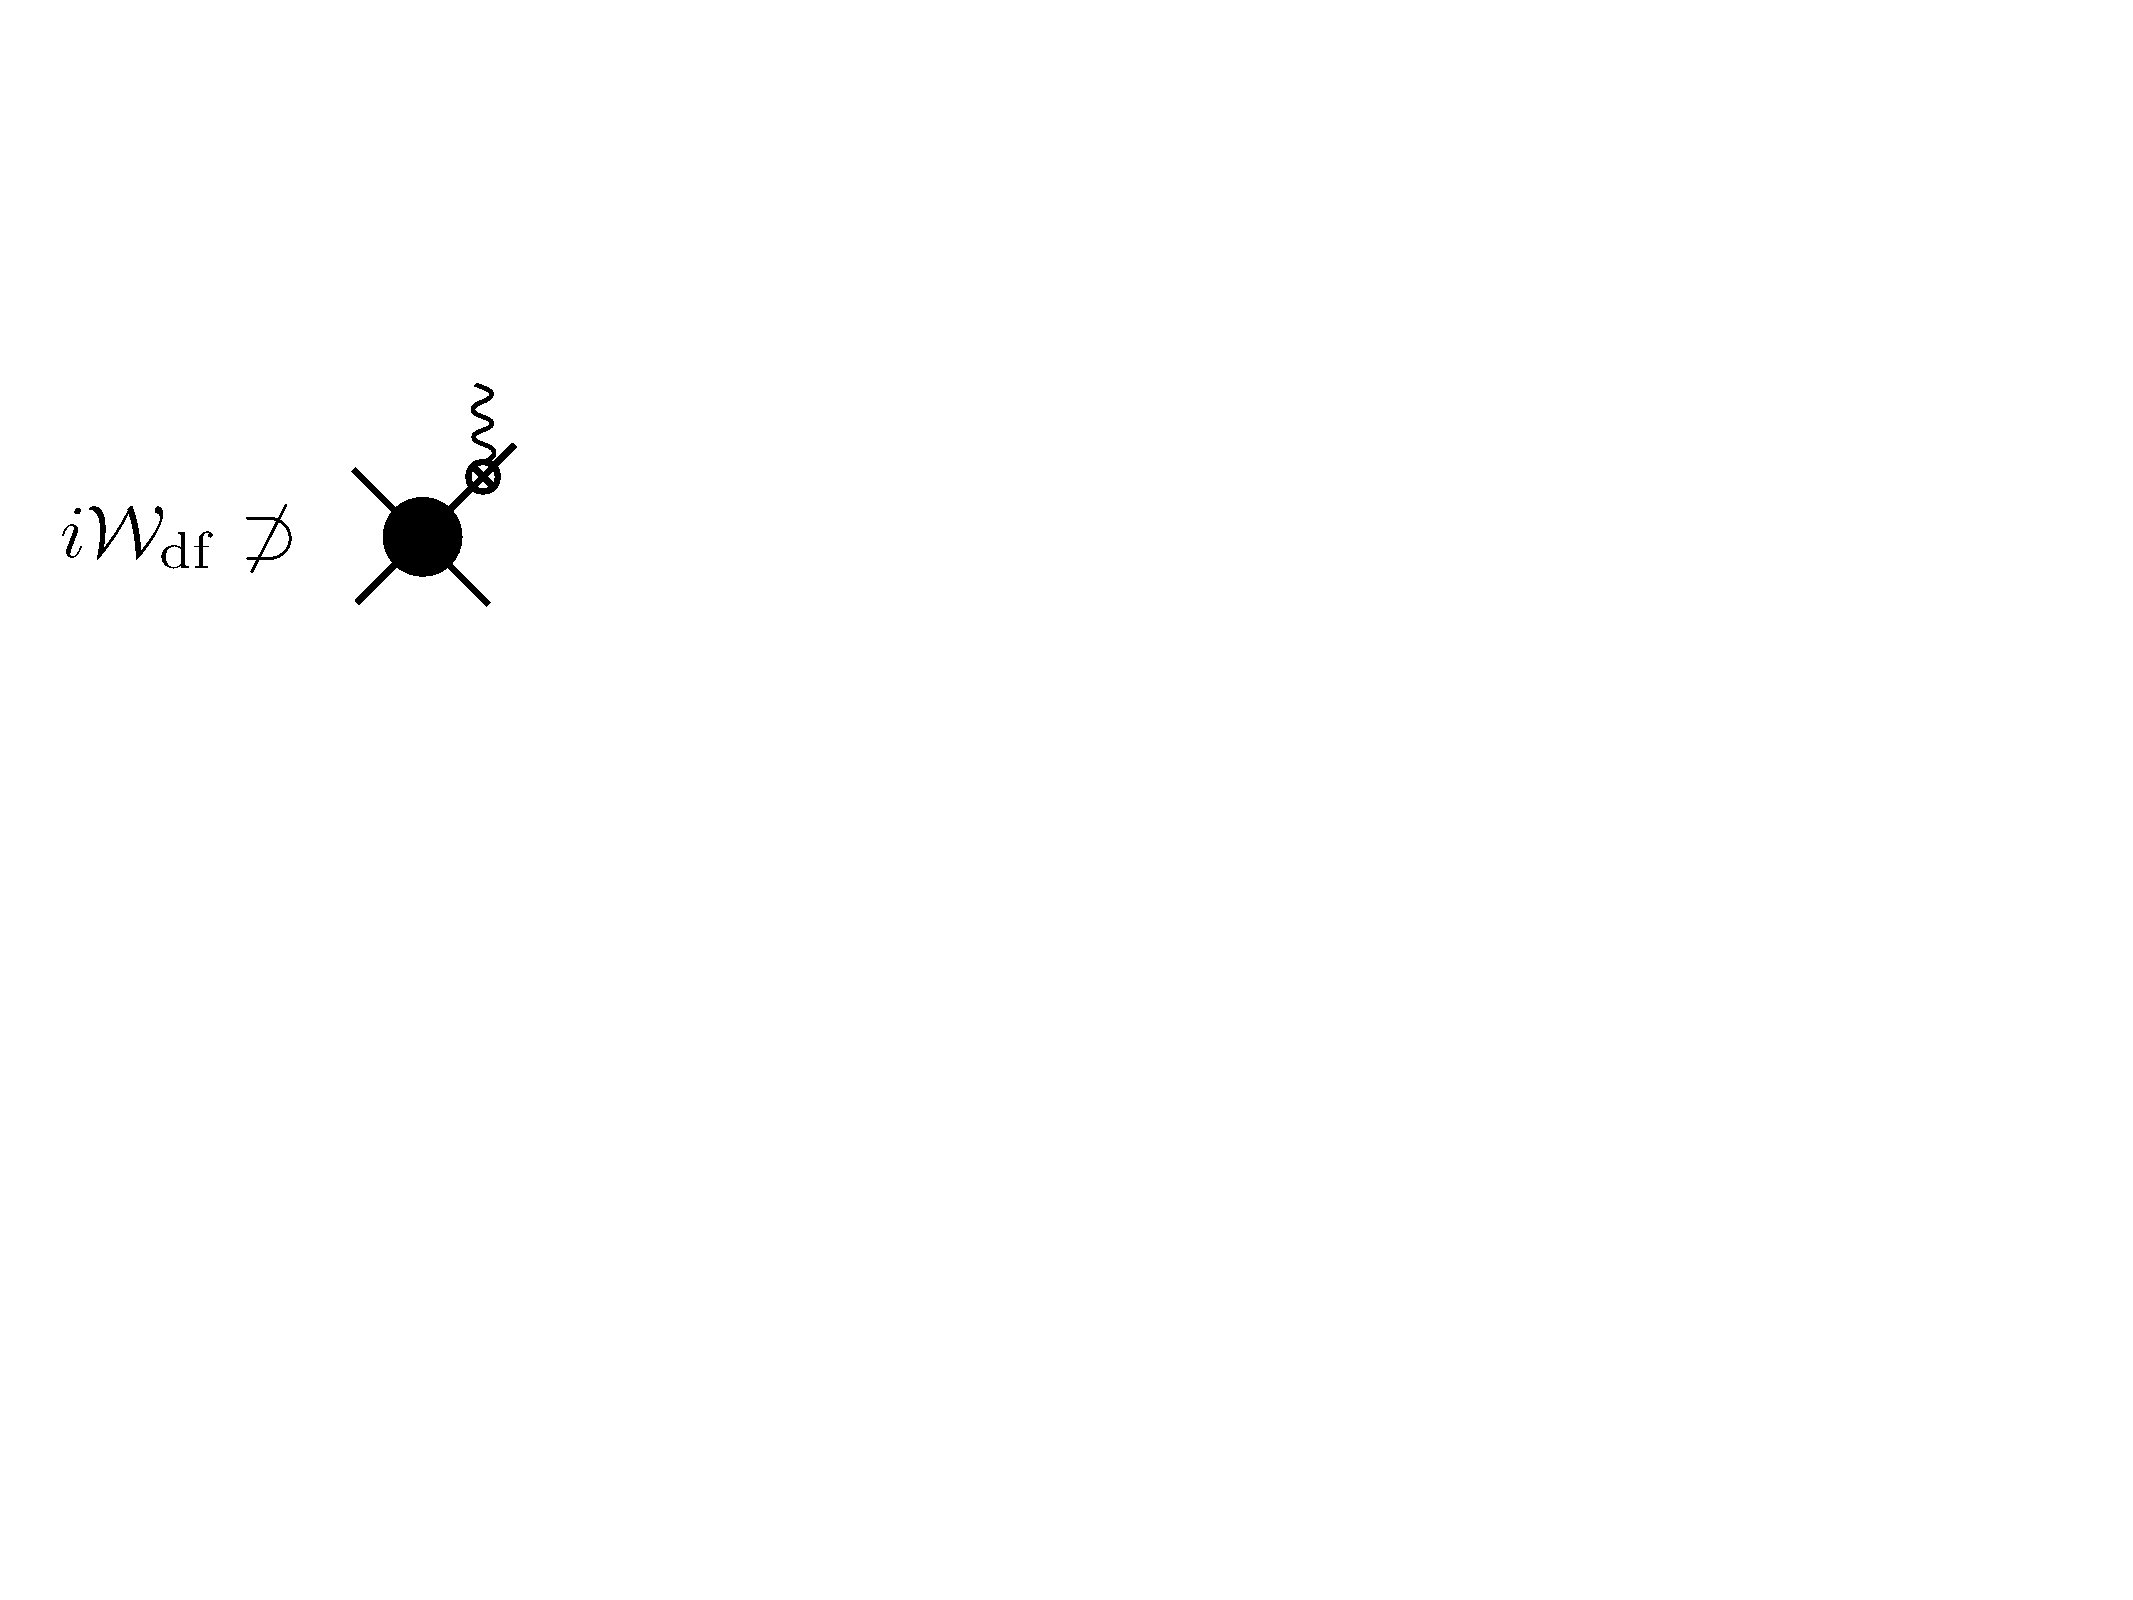
\includegraphics[scale=0.5]{figs/not_in_iWdf}}
\hspace{.5cm}
\subfigure[]{
\label{fig:IWdf_res_pole}
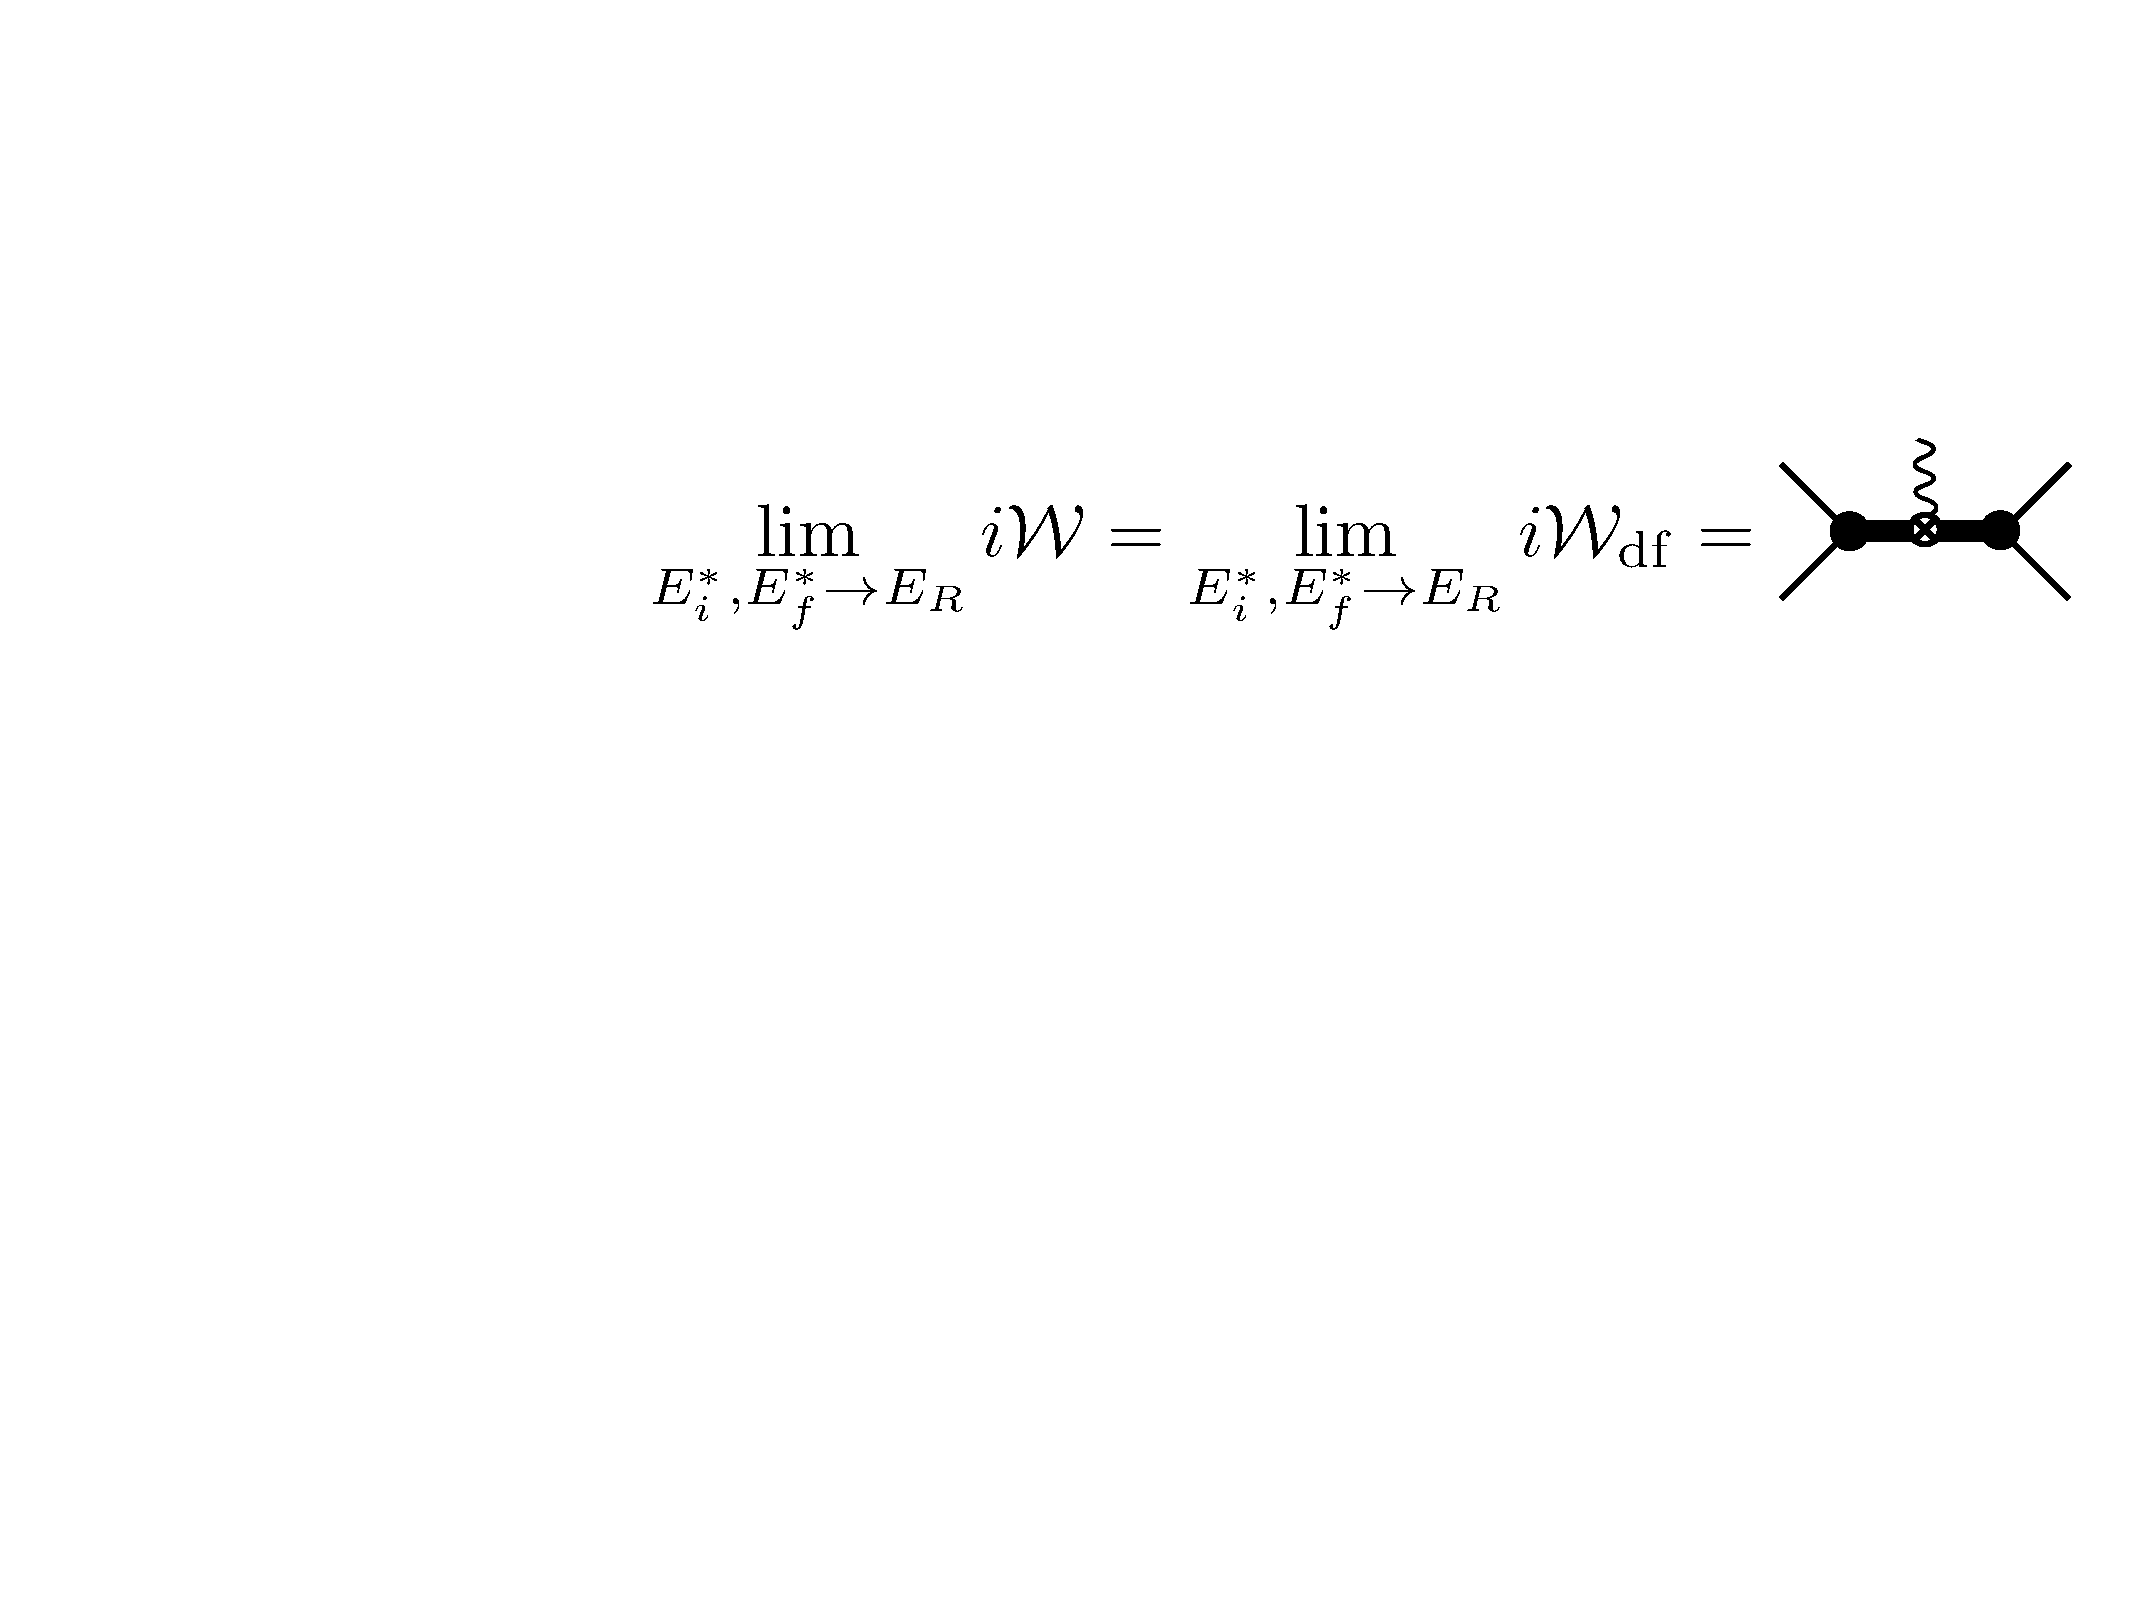
\includegraphics[scale=0.5]{figs/IWdf_res_pole}}
\caption{(a) Shown is an example of diagrams absent in $\Wdf$. (b) Shown is the postulate behavior of the $\Wdf$ near the resonance pole. }\label{fig:Wdf_pole}
\end{center}
\end{figure*}
%




\clearpage


\section{Quantization Conditions}
The relativistic scattering amplitude, $\mathcal{M}$, can be written in terms of the $S$-matrix. When there are N-channels open, both the scattering amplitude and the $S$-matrix are $N\times N$ size matrices. It is convenient to introduce a diagonal matrix, $\mathbb{P}=\text{diag}(\sqrt{\xi_1 q^{*}_1},\sqrt{\xi_2 q^{*}_2},\ldots,\sqrt{\xi_N q^{*}_N})/\sqrt{4\pi E^*}$, where $\xi_a$ is 1/2 if the two particles in the $a{th}$ channel are identical and 1 otherwise. The CM energy $E^*$ is defined in terms of total laboratory frame energy and momentum, $E$ and $\mathbf{P}$, as $E^*=\sqrt{E^2-\mathbf{P}^2}$. For the $a{th}$ channel with two mesons each having masses $m_{i,1}$ and $m_{i,2}$, the CM relative momentum is
\begin{align}
\label{momentum}
q^{*2}_a=\frac{1}{4}\left(E^{*2}-2(m_{a,1}^2+m_{a,2}^2)+\frac{
(m_{,1}^2-m_{a,2}^2)^2}{E^{*2}}\right),
\end{align}
which simplifies to $\frac{E^{*2}}{4}-m_{a}^2$ when $m_{a,1}=m_{a,2}=m_{a}$. With this, the scattering amplitude can be written as 
\begin{align}
\label{eq:relscatamp}
i\mathcal{M}&=\mathbb{P}^{-1}~(S-\mathbb{I}_N)~\mathbb{P}^{-1},\\
%\Rightarrow S&=\mathbb{I}_N+i\mathbb{P}\mathcal{M}\mathbb{P}
\end{align}
where $\mathbb{I}_N$ is the N-dimensional identity. 
 
When a single channel is open, composed of a spinless particles, the S-matrix is a diagonal unitary matrix. The diagonal elements correspond to the different angular momenta that the two particles can carry.  Conservation of angular momentum requires the S-matrix to be diagonal in $\ell$. Azimuthal symmetry tells us that all $m$ components are identical. In summary, the S-matrix satisfies the following expression,
\begin{eqnarray}
\mathcal{S}_{\ell,m;\ell',m'}
=\delta_{\ell\ell'}\,\delta_{m m'}\,\mathcal S_{\ell}.
\end{eqnarray}
 which can be parametrized by a single function, the scattering phase shift,
 \begin{align}
 S_{\ell}=e^{2i\delta_\ell}.
\end{align}
From this and Eq.~\ref{eq:relscatamp}, one can arrives at 
 \begin{align}
\mathcal M_{\ell}=\frac{8\pi E^*}{\xi}\frac{1}{q^*\cot\delta_{\ell}-iq^*} \,.
\label{eq:scatamp}
 \end{align}
{\raul [Task \#1: Proof this]}
 
 
The master equation that defines the relationship between the finite volume spectrum and the infinite volume scattering parameters is \cite{Luscher:1986pf, Rummukainen:1995vs, Kim:2005gf, Briceno:2012yi, Hansen:2012tf, Briceno:2014oea}
\begin{align}
\det[F^{-1}(P,L) + \mathcal M(P)]=
{\rm{det}}_{\rm{oc}}\left[\rm{det}_{\rm{pw}}\left[F^{-1}(P,L) + \mathcal M(P)\right]\right]=0 \,.
\label{eq:QC}
\end{align}

where the determinant $\rm{det}_{\rm{oc}}$ is over the N open channels and the determinant $\rm{det}_{\rm{pw}}$ is over the partial waves, and both $\mathcal{M}$ and $\delta \mathcal{G}^V$ functions are evaluated on the on-shell value of the momenta. $F$ is a diagonal matrix in the number of open channels, but it is non-diagonal in angular momentum, 
\begin{equation}
\label{eq:Fscdef}
F_{a \ell m ; a' \ell' m'}(P,L)  \equiv \delta_{aa'}\xi_a 
\left[\frac{1}{L^3}\sum_{\mathbf{k}}\hspace{-.5cm}\int~\right]
\frac{ 4 \pi  Y_{\ell m }(\hat {\textbf k}^*_a)Y^*_{\ell' m'}(\hat {\textbf k}^*_a)  }{2 \omega_{a1} 2 \omega_{a2}(E -  \omega_{a1} - \omega_{a2} + i \epsilon )} \left (\frac{k^{*}_a}{q^*_a} \right)^{\ell+\ell'} \,,
\end{equation}
where we are adopting the compact notation of Ref.~\cite{Briceno:2015tza}
\begin{equation}
 \left[ \frac{1}{L^3}\sum_{\mathbf{k}}\hspace{-.5cm}\int~\right]f(\textbf{k})\equiv\bigg [ \frac{1}{L^3} \sum_{\textbf k \in (2 \pi/L) \mathbb Z^3} - \int \frac{d\textbf k}{(2 \pi)^3} \bigg ] f(\textbf{k})\,.
\end{equation}


In Sec.~\ref{app:Fnum} we show that this can be written as 
\begin{equation}
F_{a \ell m,a' \ell' m'}(P,L)= \delta_{aa'}\frac{iq^*_a}{8\pi E^*}\xi_a \left[\delta_{\ell\ell'}\delta_{m m'} +i\sum_{\ell'' m''}\frac{(4\pi)^{3/2}}{q_a^{*({\ell''}+1)}}c_{a \ell'' m''}^{{\pmb \Delta}}(q_a^{*2};{L})  \int d\Omega~Y^*_{ \ell m}(\hat {\textbf k}^*_a) Y^*_{\ell'' m''}(\hat {\textbf k}^*_a) Y_{\ell' m'}(\hat {\textbf k}^*_a) \right],
\label{eq:Ffunct_KSS}
\end{equation}
where $\Delta \equiv \frac{\textbf P L}{2 \pi} \left (1 + \frac{m_{a1}^2 - m^{a2}_2}{E^{*2}} \right)$ and $c_{a \ell'' m''}^{{\pmb \Delta}}$ are defined in Sec.~\ref{app:Fnum}.

In this work, we will primarily be focused on the case where there is a single channel open composed of two spinless particles that are degenerate. In particular, we will only consider $\pi\pi$ systems, with emphasis on the $\rho$ channel. This means that $\Delta \equiv \frac{\textbf P L}{2 \pi} =\textbf{d}$. Given that it will be surpperflous will drop the channel index $``a"$. Finally, in this limit the determinant appearing in Eq.~\ref{eq:QC} reduces to one over partial waves alone
\begin{align}
\det[F^{-1}(P,L) + \mathcal M(P)]=
\rm{det}_{\rm{pw}}\left[F^{-1}(P,L) + \mathcal M(P)\right]=0 \,.
\label{eq:QC_onech}
\end{align}


%and the function $c^{\textbf{P}}_{lm}$ is defined as~\cite{Davoudi:2011md, Fu:2011xz, Leskovec:2012gb}
% \begin{align}
% 	c^\mathbf{d}_{lm}(q^{*2};L)=\frac{\sqrt{4\pi}}{\gamma L^3}\left(\frac{2\pi}{L}\right)^{l-2}\mathcal{Z}^\mathbf{d}_{lm}[1;(k^*_j {L}/2\pi)^2],
%\hspace{1cm} 
%\mathcal{Z}^\mathbf{d}_{lm}[s;x^2]=\sum_{\mathbf{n}}\frac{\mathbf{r}^lY_{l,m}(\mathbf{r}_n)}{(r^2_n-x^2)^s},
%\end{align}
%%
%where $\mathbf{\mathbf{r}_n}=\frac{1}{\gamma}(\mathbf{n}_{||}-\alpha\mathbf{d})+\mathbf{n}_{\perp}$, $\gamma=E/E^*$, $E=\sqrt{P^2+E^{*2}}$, $\mathbf{n}$ is an integer triplet, $\mathbf d$ is the normalized boost vector $\mathbf d=\mathbf{P}L/2\pi$, and $\alpha=\frac{1}{2}\left[1+\frac{m_1^2-m_2^2}{E^{*2}}\right]$.
%The numerical evaluation $\mathcal{Z}$-function can be accelerated by writting it as~\cite{Leskovec:2012gb}
% \begin{align}
%\mathcal{Z}^\mathbf{d}_{lm}[1;x^2]&=\sum_{\mathbf{n}}\frac{e^{- (r^2_n-x^2)}}{r^2_n-x^2}\mathbf{r}_n^lY_{l,m}(\mathbf{r}_n)
%+\delta_{l,0}~Y_{00}~\gamma~\pi^{3/2}~\left[2x^2\int^{1}_0dt\frac{e^{tx^2}}{\sqrt{t}}-2{e^{ x^2}}\right]\nonumber\\
%&+~\gamma~i^l\sum_{\mathbf{w}\neq0}~e^{i2\pi\alpha\mathbf{w}\cdot \mathbf{d}}~|\hat{\gamma}\mathbf{w}|^l~Y_{l,m}(\Omega_{\hat{\gamma}\mathbf{w}})\int^{1}_0dt\left(\frac{\pi}{t}\right)^{3/2+l}e^{tx^2}e^{-\pi^2|\hat{\gamma}\mathbf{w}|^2/t}
%\end{align}
%where 
%\begin{align}
%\hat{\gamma}\mathbf{w}={\gamma}\mathbf{w}_{||}+\mathbf{w}_{\perp}.
%\end{align}
%
%
%Note, both $\textbf{n}$ and $\textbf{w}$ are integer triplets. For example, $\textbf{n}=(n_x,n_y,n_z)$, where each $n_i$ component is an integer running from negative infinity to positive infinity. $\mathbf{w}_{||}$ and $\mathbf{w}_{\perp}$ are defined such that they are parallel and orthogonal to the boost vector, $\textbf{d}$, respectively. In other words, $\mathbf{w}_{\perp}\cdot\textbf{d}=0$, and $\mathbf{w}_{||}=(\mathbf{w}\cdot\textbf{d})\,\textbf{d}=0$.

  


 %%%%%%%%%%%%%%%%%%%%%%%%%%%%%%%%%%%%%%%%%%
\subsection{Simplification for $\pi\pi$ in the S- and P-wave channels}
%%%%%%%
\begin{center}
\begin{table} 
\begin{tabular}{ c c c c} 
\hspace{.1cm}\textbf{d}\hspace{.1cm}& 
 \hspace{.1cm}$(00n)$\hspace{.1cm}& 
 \hspace{.1cm}$(nn0)$\hspace{.1cm}& 
 \hspace{.1cm}$(nnn)$\hspace{.1cm}
 \\\hline
& $\alpha_{20,\mathbb{A}_1}^\mathbf{d} =\frac{2}{\sqrt{5}}$
& $\alpha_{20,\mathbb{A}_1}^\mathbf{d} =-\frac{1}{\sqrt{5}},\hspace{.5cm}
\alpha_{22,\mathbb{A}_1}^\mathbf{d} =-i\sqrt{\frac{6}{5}}$
& $\alpha_{22,\mathbb{A}_1}^\mathbf{d} =-2i\sqrt{\frac{6}{5}}$
 \\ 
 & $\alpha_{20,\mathbb{E}}^\mathbf{d} =-\frac{1}{\sqrt{5}}$
  & 
 $\alpha_{20,\mathbb{B}_1}^\mathbf{d} =-\frac{1}{\sqrt{5}},\hspace{.5cm}
  \alpha_{22,\mathbb{B}_1}^\mathbf{d} =i\sqrt{\frac{6}{5}}$
 & $\alpha_{22,\mathbb{E}}^\mathbf{d} =i\sqrt{\frac{6}{5}}$\\
 && 
 $\alpha_{20,\mathbb{B}_2}^\mathbf{d} =\frac{2}{\sqrt{5}}$
\vspace{.05cm}\\ \hline
\end{tabular}
\caption{Nonzero values of $\alpha_{20,\Lambda}^\mathbf{d}$ and $\alpha_{22,\Lambda}^\mathbf{d}$ for ${\mathbf{d}^2}\leq3$. For the $\mathbb{T}_1^-$ irrep of ${O}^D_h$, the $c^\mathbf{d}_{2m}$ vanish, therefore there is no need to define $\alpha_{2m,\Lambda}^\mathbf{d}$ for this irrep. 
}
\label{table:alphad}
\end{table}
\end{center} 

Let us consider the low-energy behavior of the quantization condition. In particular, we will consider the case where the  the scattering amplitude is dominated by a single angular momentum. Furthermore, given that the $\pi\pi$ must satisfy Bose statistics, they must have a totally symmetric wavefunction. If we consider the isoscalar ($I=0$) or isotensor ($I=2$) channels, where the isospin component of the wavefunction is symmetric, the orbital angular momenta must be even ($\ell=0,2,4,\ldots$). Equivalently, for the isotriplet channel ($I=1$), the angular momenta must be odd even ($\ell=1,3,5,\ldots$). Some particularly interesting examples, are the $\sigma$ resonance, which couples to the couples to the $(I,\ell)=(0,0)$ channel~\cite{Briceno:2016mjc}, and the $\rho$ resonance which couples to the $(I,\ell)=(1,1)$ channel~\cite{Wilson:2015dqa, Dudek:2012xn}. 

First, let us consider the case where the scattering amplitude is dominated by the S-wave, in other words, 
 \begin{align}
 \hspace{-2cm}
\mathcal M
\approx
\left(
\begin{array}{cccccc}
 \mathcal M_{0} 
 \\
& 0
 \\
&& 0
 \\
&&&0
\\
&&&& \ddots
\\
\end{array}
\right). \hspace{1cm}
 \end{align}
Inserting this into Eq.~\ref{eq:QC}, one can show that the quantization condition is fairly simple
\begin{align}
q^{*}\cot\delta_{S}-
{4\pi}
 c^\mathbf{d}_{00}(q^{*2};L)=0.
 \label{eq:Swave}
\end{align}
{\raul [Task \#2: Proof this]}

The P-waves quantization conditions are only slightly more complicated. First, we need to remember that the $\ell=1$ angular momentum is a three-dimensional irrep of the $\mathcal{O}(3)$ group. This implies that the scattering amplitude has three identical components
 \begin{align}
 \hspace{-2cm}
\mathcal M
\approx
\left(
\begin{array}{cccccc}
  0
 \\
& \mathcal M_{1} 
 \\
&& \mathcal M_{1} 
 \\
&&&\mathcal M_{1} 
\\
&&&& \ddots
\\
\end{array}
\right). \hspace{1cm}
 \end{align}
 Inserting these into Eq.~\ref{eq:QC} and block-diagonalizing the matrix inside the determinant, one finds that for each boost vector, $\mathbf{d}$, there are three quantization conditions describing the spectrum. For the symmetry group we will be considering, these can be compactly written as, 
\begin{align}
q^{*}\cot\delta_{P}-
{4\pi}\left(
 c^\mathbf{d}_{00}(q^{*2};L)
+\frac{\alpha_{20,\Lambda}^\mathbf{d}}{q^{*2}} c^\mathbf{d}_{20}(q^{*2};L)
+\frac{\alpha_{22,\Lambda}^\mathbf{d}
}{q^{*2}} c^\mathbf{d}_{22}(q^{*2};L)
\right)=0
\end{align}
where the values of $\alpha_{2m,\Lambda}^\mathbf{d}$ are shown in Table~\ref{table:alphad}. 


When the system is at rest $\alpha_{2m,\Lambda}^\mathbf{d}=0$, there is a single irrep of the cubic group which couples to P-wave channel. This is the $\mathbb{T}_1^-$ irrep, which is three-dimensional. Given that the three-components of the $\mathbb{T}_1^-$ irrep are necessarily degenerate, only one QC is needed to describe its spectrum, which resembles that of the S-wave,
\begin{align}
\mathbb{T}_1^-:\hspace{.5cm} q^{*}\cot\delta_{P}-
{4\pi}
 c^\mathbf{d}_{00}(q^{*2};L)=0.
\end{align}
When you boost the system along the z-axis, you get two different irreps, the $\mathbb{A}_1$ and $\mathbb{E}$. Note, the $\mathbb{A}_1$ is one-dimensional and $\mathbb{E}$ is two-dimensional. More technically, the $\mathbb{A}_1$ couples only to the helicity-0 components of the P-wave amplitude, while $\mathbb{E}$ couples to the helicity 1 and -1 components. The two irreps have  distinct spectra satisfying,
\begin{align}
\mathbb{A}_1&:\hspace{.5cm}q^{*}\cot\delta_{P}-
{4\pi}
 c^\mathbf{d}_{00}(q^{*2};L)
 -
\frac{2}{\sqrt{5}}\frac{4\pi}{q^{*2}}
 c^\mathbf{d}_{20}(q^{*2};L)=0\\
\mathbb{E}&:\hspace{.5cm}q^{*}\cot\delta_{P}-
{4\pi}
 c^\mathbf{d}_{00}(q^{*2};L)
 +
\frac{1}{\sqrt{5}}\frac{4\pi}{q^{*2}}
 c^\mathbf{d}_{20}(q^{*2};L)=0. 
\end{align}
Note, the two components of the $\mathbb{E}$ are degenerate. 

Similarly, for the other irreps. 
\section{Relating the finite-volume matrixs element to $\pi\pi\gamma^\star\to\pi\pi$ amplitude}

 \begin{equation}
\Big | \langle E_{n_f}, \textbf P_f, L \vert  \mathcal J(0)  \vert E_{n_i}, \textbf P_i, L \rangle \Big |^2_L 
=\frac{1}{L^6} {\rm{Tr}}\left[
 \mathcal R(E_{n_i}, \textbf P_i) 
\Wtildf(P_i,P_f,L)
\mathcal R(E_{n_f}, \textbf P_f)  
\Wtildf(P_f,P_i,L)
\right] \,.
  \label{eq:2to2_notdegen}
\end{equation}

\begin{equation}
\label{eq:WtiltoWdf}
 \Wtildf(P_f,P_i,L)  \equiv \Wdf(P_f,P_i) +  \mathcal  M(P_f) \ [G(L) \cdot \w](P_f,P_i) \ \mathcal M(P_i)  \,.
 \end{equation}

where $\omega$ is the one-body amplitude (closely related to the pion form factor)
\begin{align}
\label{eq:Rdef}
\mathcal R(E_{n}, \textbf P) &\equiv  \lim_{P_4 \rightarrow i E_{n}} \left[ - (i P_4 + E_{n}) \frac{1}{F^{-1}(P,L) + \mathcal M(P)}\right] \,.
%%%%%%%%%%%%%%%%%%%%%%%%%%%%%%%%%%%%%%%%%%%%%
%%%%%%%%%%%%%%%%%%%%%%%%%%%%%%%%%%%%%%%%%%%%%
\\
\label{eq:Gdotw}
 [G(L) \cdot \w]_{a \ell_fm_{f}; b\ell_im_{i}}(P_f,P_i) 
 &\equiv 
\sum_{s,t=1,2}  \xi_a \xi_b  G^{st}_{a \ell_f m_{f}, a' \ell_f' m_{f}'; b' \ell_i' m_{i}', b \ell_i m_{i}}(P_f,P_i,L) 
~\w_{a'sb't; \ell_f' m_{f}';  \ell_i' m_{i}'}(P_f;P_i)  \,.
\end{align} 
and
 \begin{multline}
\label{eq:Gmat}
G^{st}_{a \ell_f m_{f},a' \ell_f' m_{f}'; b' \ell_i' m_{i}', b \ell_i m_{i}}(P_f,P_i,L)  \equiv \\
\hspace{-4cm}
\delta_{aa'} \delta_{bb'}
\left[\frac{1}{L^3}\sum_{\mathbf{k}}\hspace{-.5cm}\int~\right]
~\frac{1}{2\omega_{a\slashed s}}
\frac{ 4 \pi  Y_{\ell_fm_{ f}}(\hat {\textbf k}^*_{af})
Y^*_{\ell_f'm_{f}'}(\hat {\textbf k}^*_{af})
 }{2 \omega_{{asf}}(E_f -  \omega_{a\slashed s} - \omega_{asf} + i \epsilon )} 
  \bigg (\frac{k^{*}_{af}}{q^*_{af}} \bigg)^{\ell_f+\ell_f'}
\frac{ 4 \pi  Y_{\ell_i' m_{i}'}(\hat {\textbf k}^*_{bi})
Y^*_{\ell_i m_{i}}(\hat {\textbf k}^*_{bi})
 }{2 \omega_{bti}(E_i -  \omega_{b\slashed t} - \omega_{bti} + i \epsilon )} 
 \bigg (\frac{k^{*}_{bi}}{q^*_{bi}} \bigg)^{\ell_i+\ell_i'}
  \,.
\end{multline}

Here we have a list of things to do, 

\begin{itemize}
\item Simplify these expressions for the single channel case, degenerate masses, etc
\item I think we might want to write things in terms of $G(L) \cdot \w$ in the first place. This avoid introducing a weird spherical harmonic decomposition of $\w$. 
\end{itemize}


 %%%%%%%%%%%%%%%%%%%%%%%%%%%%%%%%%%%%%%%%%%%%%%
 \subsection{Subduction}
 
%%%%%%%%%%%%%%%%%%%%%%%%%%%%%%%%%%%%%%%%%%
\subsection{Simplifying limits}

\label{sec:simplim}

In this section we consider various simplifying limits of the general result, derived in the last section. We begin by taking the energies considered to be very close to the lowest two-particle threshold.   In this case, the infinite-volume quantities $\w$, $\mathcal M$ and $\Wdf$ are all dominated by their S-wave values. We thus drop all higher partial waves in the matrices $w_{a1b1; \ell' m'; \ell  m }(P_f,P_i)$, $\mathcal M_{ab; \ell' m'; \ell m}(P)$ and $\mathcal W_{\mathrm{df};ab;\ell' m'; \ell m}(P_f,P_i)$. The second consequence of near-threshold energies is that only the lowest two-particle channel is open. In discussing this system it is convenient to introduce the shorthand
\begin{align}
w_{11}(P_f,P_i) & \equiv w_{a1b1; 00;00 }(P_f,P_i) \,, \\
\mathcal M (P) & \equiv \mathcal M_{ab; 00; 00}(P)\,, \\
\mathcal W_{\mathrm{df}}(P_f,P_i) & \equiv \mathcal W_{\mathrm{df};ab;00;00}(P_f,P_i) \,.
\end{align}
We comment here that, for a scalar form factor, symmetry and on-shell constraints guarantee that $w$ only depends on $(P_f-P_i)^2$ and thus not on $\textbf k$. In this case, the truncation of $w$ to the S-wave is exact.  
 Since all matrices have reduced to one dimensional, the trace may be dropped from Eq.~(\ref{eq:2to2_notdegen})
\begin{equation}
\label{eq:mainresSwave}
\Big | \langle E_{n_f}, \textbf P_f, L \vert  \mathcal J(0)  \vert E_{n_i}, \textbf P_i, L \rangle \Big |^2_L 
=\frac{1}{L^6}
 \mathcal R(E_{n_i}, \textbf P_i)
\Wtildf(P_i,P_f,L) \mathcal R(E_{n_f}, \textbf P_f) 
 \Wtildf(P_f,P_i,L) \,.
\end{equation}
 In addition, the residue matrix $\mathcal R$ simplifies significantly
\begin{align}
\mathcal R(E_{n}, \textbf P) & =   \left [ \frac{\partial}{\partial E} \left( F^{-1}(P,L) + \mathcal M(P) \right ) \right ]_{E=E_n}^{-1} = -  \left [ \mathcal M^2(P) \frac{\partial}{\partial E} \left( F(P,L) + \mathcal M^{-1}(P) \right ) \right ]_{E=E_n}^{-1} \,, \\
& = - \xi \frac{q^*}{8 \pi E^*}   \left [ \sin^2\! \delta\ e^{ 2i \delta}\  \frac{\partial}{\partial E} \left( \cot\phi^\textbf{d}_{}+ \cot\delta \right ) \right ]_{E=E_n}^{-1}    \,, \\
& = \xi \frac{q^*}{8 \pi E^*} e^{-2i \delta}  \left [  \frac{\partial}{\partial E} \left( \phi^\textbf{d}_{} + \delta \right ) \right ]_{E=E_n}^{-1}    \,,
 \end{align}
where $F = F_{a00;b00}$ is understood and where we have introduced the S-wave L\"uscher pseudophase
 \begin{equation}
 \cot \phi^{\textbf d} = \xi \frac{q^*}{8 \pi E^*} \mathrm{Re}F(P,L) \,.
 \end{equation}
Here we have also used the relation between scattering amplitude $\mathcal M$ and scattering phase shift $\delta$, given in Eq.~(\ref{eq:scatamp}) above. Substituting this result for $\mathcal R$ into Eq.~(\ref{eq:mainresSwave}) and rearranging gives
 \begin{multline}
 \label{eq:swaveWtoFV}
\Big [ e^{-i \delta_i}
\Wtildf(P_i,P_f,L) e^{- i \delta_f} \Big ] \Big [ e^{- i \delta_f}  \Wtildf(P_f,P_i,L) e^{- i \delta_i} \Big ]
\\[5pt] = \frac{8 \pi E^*_f}{q^*_f \xi} \frac{8 \pi E^*_i}{q^*_i \xi}  \left [  \frac{\partial}{\partial E_f} \left( \phi^\textbf{d} + \delta \right ) \right ]_{E_f=E_{f,n}} \left [  \frac{\partial}{\partial E_i} \left( \phi^\textbf{d} + \delta \right ) \right ]_{E_i=E_{i,n}} L^6 \Big | \langle E_{n_f}, \textbf P_f, L \vert  \mathcal J(0)  \vert E_{n_i}, \textbf P_i, L \rangle \Big |^2_L 
 \,.
\end{multline}
We thus see that a naive Lellouch-L\"uscher-like proportionality factor arises between the finite- and infinite-volume quantities. Since the right-hand side of this expression is manifestly pure real, this result also suggest a Watson-like theorem for $\Wtildf$, namely that its complex phases are the strong scattering phases associated with the incoming and outgoing two-particle states. 
 %%%%%%%%%%%%%%%%%%%%%%%%%%%%%%%%%%%%%%%%%%
\section{Numerical evaluation of the relevant geometric functions}
\subsection{Numerically evaluating $F$}
 
 \label{app:Fnum}
 
 Here I am stealing content from Ref.~\cite{Briceno:2015tza}, where we give some detail between the different expressions for the F-function. First, let us equate the expressions give in Eq.~\ref{eq:Fscdef} and Eq.~\ref{eq:Ffunct_KSS}. To do this, we will explicitly separate the real and imaginary parts of the propagator. The imaginary component is given by the $i \epsilon$ prescription.  We do this using 
\begin{align}
\label{eq:PVdef}
\frac{1}{2 \omega_{a2}(E -  \omega_{a1} - \omega_{a2} + i \epsilon )}
= \frac{\omega_{a1}^*}{E^* (q_a^{*2}-k_a^{*2}+i\epsilon)} + \mathcal S_2
=\frac{\omega_{a1}^*}{E^*}\left[{\rm{P.V.}}\frac{1}{(q_a^{*2}-k_a^{*2})}-i\pi\delta(q_a^{*2}-k_a^{*2})\right] + \mathcal S_2,
\end{align}
where $\mathcal S_2$ is a smooth function that will be annihilated by the sum-integral difference. Here ${\rm{P.V.}}$ denotes the principal-value pole prescription. We further reduce the expression by combining the two spherical harmonics into one
\begin{equation}
4 \pi  Y_{\ell m}(\hat {\textbf k}^*_a)Y^*_{\ell' m'}(\hat {\textbf k}^*_a) =
{4 \pi}\sum_{\ell''m''}
  Y_{\ell'' m''}(\hat {\textbf k}^*_a)
\int d\Omega_{\textbf p}~Y^*_{ \ell m}(\hat {\textbf p}^*_a) Y^*_{\ell'' m''}(\hat {\textbf p}^*_a) Y_{\ell' m'}(\hat {\textbf p}^*_a).
\end{equation}
Putting all the pieces together, we can rewrite Eq.~(\ref{eq:Fscdef}) as Eq.~\ref{eq:Ffunct_KSS}, where $c_{a \ell m}^{{\pmb \Delta}}(q_a^{*2};{L})$ is defined as
\begin{equation}
c_{a \ell m}^{{\pmb \Delta}}(q^{*2}_a;{L})
=
\left[\frac{1}{L^3}\sum_{\mathbf{k}}\hspace{-.5cm}\int~\right]
\frac{\omega_{a1}^*k_a^{*\ell}}{\omega_{a1}}
{\rm{P.V.}}\frac{ \sqrt{4 \pi}  Y_{\ell m}(\hat {\textbf k}^*_a)  }{  k_a^{*2}-q_a^{*2}}.
\end{equation}
Alternatively, this function can be written in terms of the generalized Zeta functions~\cite{Kim:2005gf}
\begin{eqnarray}
\label{eq:clm}
c^{\pmb \Delta}_{a\ell m}(q_a^{*2}; {L})
=\frac{\sqrt{4\pi}}{\gamma L^3}\left(\frac{2\pi}{L}\right)^{\ell-2}\mathcal{Z}^{\pmb \Delta}_{a\ell m}[1;(q_a^* {L}/2\pi)^2],
\hspace{1cm}
\mathcal{Z}^{\pmb \Delta}_{a \ell m}[s;x^2]
= \sum_{\mathbf r \in {\mathcal P}_{{\pmb \Delta}}}\frac{{r}^\ell Y_{\ell m}(\hat {\mathbf{r}})}{(r^2-x^2)^s} \label{eq:clm} \,,
\end{eqnarray} 
where 
\begin{align}
P_{\pmb \Delta} & \equiv  \bigg \{  \, \textbf r \ \bigg \vert \ \textbf r =   \pmb \gamma^{-1}\left( \textbf n - \frac12 \pmb \Delta \right) \,, \ \textbf n \in \mathbb Z^3 \bigg \} \,, \\
\pmb \Delta & \equiv \frac{\textbf P L}{2 \pi} \left (1 + \frac{m_{a1}^2 - m_{a2}^2}{E^{*2}} \right) \,, \\
\pmb \gamma^{-1} \textbf p & \equiv \gamma^{-1} \textbf p_{\parallel} + \textbf p_{\bot} = (E/E^*)^{-1} \textbf p_{\parallel} + \textbf p_{\bot}  \,,
\end{align}
and where $\textbf p_{\parallel}$ and $\textbf p_{\bot}$ are the parallel and perpendicular components of $\textbf p$ with respect to the fixed total momentum $\textbf P$. We close by giving a particularly efficient form for evaluating these quantities~\cite{Leskovec:2012gb},
\begin{multline}
Z_{a\ell m}^{\pmb \Delta}(1,x^2) = \sum_{\textbf r \in P_{\pmb \Delta}} \frac{ r^\ell  Y_{\ell m}(\hat {\textbf r})}{ r^2 - x^2} e^{-( r^2 - x^2)} + \gamma \frac{\pi}{2} \delta_{\ell 0} \delta_{m0} G(x) \\
+ \gamma \pi^{3/2} \int_0^1 dt \frac{e^{tx^2}}{t^{3/2}} \left( \frac{\pi i}{t} \right)^{\ell} \sum_{\textbf n \neq 0} e^{-i \pi \textbf n \cdot \pmb \Delta} \vert \pmb \gamma \textbf n \vert ^{\ell}  Y_{\ell m}( \hat {\pmb \gamma \textbf n}) e^{-(\pi \pmb \gamma \textbf n)^2/t} \,,
\end{multline}
where $\pmb \gamma \textbf p  \equiv \gamma \textbf p_{\parallel} + \textbf p_{\bot}$ and
\begin{equation}
G(x)  \equiv \int_0^1 dt \frac{e^{t x^2} - 1}{t^{3/2}}   - 2  \,.
\end{equation}

where $\alpha=\frac{1}{2}\left[1+\frac{m_1^2-m_2^2}{E^{*2}}\right]$.

{\raul [Task \#3: Write code for $\mathcal{Z}^\mathbf{d}_{lm}$. In other words, drop all of the channel indices. Also, we will only need to think about the case where the masses are degenerate.]}

{\raul [Task \#4: Compare to Eq. 70 in https://arxiv.org/pdf/1202.2145.pdf]}

{\raul [Task \#5: Derive Eq. 70 starting from Eq. 59 in https://arxiv.org/pdf/1202.2145.pdf]}



  %%%%%%%%%%%%%%%%%%%%%%%%%%%%%%%%%%%%%%%%%%
 \subsection{Numerically evaluating $G$}


\label{app:Gnum}

 

\subsubsection{Introduction and general definition \label{sec:Gfunc}}
The goal of this project is to calculate infinite-volume matrix elements of the from
\begin{equation}
\langle \pi \pi ; \mathrm{out}; P_f  \vert \mathcal J_\mu (0) \vert \pi \pi ; \mathrm{in}; P_i \rangle \,,
\end{equation}
where $\mathcal J_\mu$ is a vector current and the states on either side are two-particle asymptotic states with the momentum as indicated. As is described in detail in Ref.~\cite{BH2to2}, one cannot directly measure these matrix elements in a numerical lattice calculation, due to the restriction to finite volume and Euclidean time. It is however possible to extract the matrix elements by combining the following ingredients:
\begin{itemize}
\item The pion vector form factor, $F_{\pi}(Q^2)$, defined via:
\begin{equation}
\langle \pi, p_f \vert \mathcal J_\mu (0) \vert \pi , p_i \rangle = (p_f + p_i)_\mu F_{\pi}(Q^2) \bigg \vert_{Q^2 = (p_f-p_i)^2} \,.
\end{equation}
\item The finite-volume energies with two-pion quantum numbers in various moving frames: $E_n(L, \textbf P)$.
\item The finite-volume matrix elements of states with two-pion quantum numbers in various moving frames:
\begin{equation}
\langle E_{n_f}, \textbf P_f , L \vert \mathcal J_\mu (0) \vert E_{n_i}, \textbf P_i , L \rangle \,.
\end{equation}
\end{itemize}


In order to combine these ingredients and extract the desired quantity, one must calculate a new kinematic function called $G$ and defined by
\begin{multline}
G_{a \ell_f m_{f},a' \ell_f' m_{f}'; b' \ell_i' m_{i}', b \ell_i m_{i}}(P_f,P_i,L)  \equiv \\
\hspace{-4cm}
\delta_{aa'} \delta_{bb'}
\left[\frac{1}{L^3}\sum_{\mathbf{k}}\hspace{-.5cm}\int~\right]
~\frac{1}{2\omega_{a1}}
\frac{ 4 \pi  Y_{\ell_fm_{ f}}(\hat {\textbf k}^*_{af})
Y^*_{\ell_f'm_{f}'}(\hat {\textbf k}^*_{af})
 }{2 \omega_{{a2f}}(E_f -  \omega_{a1} - \omega_{a2f} + i \epsilon )} 
  \bigg (\frac{k^{*}_{af}}{q^*_{af}} \bigg)^{\ell_f+\ell_f'}
\frac{ 4 \pi  Y_{\ell_i' m_{i}'}(\hat {\textbf k}^*_{bi})
Y^*_{\ell_i m_{i}}(\hat {\textbf k}^*_{bi})
 }{2 \omega_{b2i}(E_i -  \omega_{b1} - \omega_{b2i} + i \epsilon )} 
 \bigg (\frac{k^{*}_{bi}}{q^*_{bi}} \bigg)^{\ell_i+\ell_i'}
  \,.
\end{multline}
To evaluate this one takes $E_i, \textbf P_i, E_f, \textbf P_f, L$ and the masses as inputs. For a given point in the summation and integration space, $\textbf k$ should also be viewed as an input. Given these quantities one must first determine $q^{*}_{bi}$, $q^{*}_{af}, k_{bi}^*, k_{af}^*, \hat {\textbf k}^*_{bi}, \hat {\textbf k}^*_{af}$ and the $\omega$s via
\begin{gather}
\sqrt{E_i^2 - \textbf P_i^2} = \sqrt{m_{b1}^2 + q^{*2}_{bi}} + \sqrt{m_{b2}^2 + q^{*2}_{bi}} \,, \hspace{30pt} \sqrt{E_f^2 - \textbf P_f^2} = \sqrt{m_{a1}^2 + q^{*2}_{af}} + \sqrt{m_{a2}^2 + q^{*2}_{af}} \,, \\[5pt]
\begin{pmatrix} \omega_{b1}^* \\ \textbf k_{bi}^*  \end{pmatrix}^{\mu} ={ \Lambda^{\mu}}_{\nu}(- \textbf P_i /E_i) \begin{pmatrix} \omega_{b1} \\ \textbf k   \end{pmatrix}^{\nu} \,, \hspace{30pt} \begin{pmatrix} \omega_{a1}^* \\ \textbf k_{af}^*  \end{pmatrix}^{\mu} ={ \Lambda^{\mu}}_{\nu}(- \textbf P_f /E_f) \begin{pmatrix} \omega_{a1} \\ \textbf k  \end{pmatrix}^{\nu}  \,, \\[5pt]
\omega_{b1} = \sqrt{m_{b1}^2 + \textbf k^2}\,, \ \ \omega_{b2i}  = \sqrt{m_{b2}^2 + (\textbf P_i - \textbf k)^2 } \,, \hspace{30pt} \omega_{a1} = \sqrt{m_{a1}^2 + \textbf k^2}\,, \ \ \omega_{a2f}  = \sqrt{m_{a2}^2 + (\textbf P_f - \textbf k)^2 } \,,
\end{gather}
where ${ \Lambda^{\mu}}_{\nu}(- \textbf P_i /E_i)$ is the boost matrix that takes the four-vector $(E_i, \textbf P_i)$ to its zero-momentum frame. From here one has all building blocks for the integrand and it remains only to sum and integrate.

{\mh [For $M_\pi L =4$, $\textbf P_i = 2 \pi \hat {\textbf z}/L$, $\textbf k = 2 \pi (1,1,0)/L$ calculate $\textbf k^*_i/M_\pi$ as a function of $E_i$.]}

\subsubsection{Reduction for two-pion states}


Here we consider the simplifications that arise for two-pion states. We find it useful to work with the target quantity $[G(L) \cdot w]$, where $w$ is the matrix element of the vector current with single-pion states 
\begin{equation}
w_\mu(P_f - k, P_i - k) \equiv
 \langle \pi; P_f - k \vert \mathcal J_\mu (0) \vert  \pi ; P_i - k \rangle \,, 
\end{equation}
and the $\cdot$ indicates that $w$ is decomposed in spherical harmonics and its indices are contracted with those in $G(L)$. Using Lorentz invariance and current conservation we can rewrite
\begin{equation}
w_\mu(P_f - k, P_i - k) 
  =  (P_f - k + P_i - k)_\mu \  F_\pi (Q^2) \,,
\end{equation}
where $Q^2 = (P_f - P_i)^2$. {\mh [Prove this result.]} Note that the pions are on shell, meaning that $(P_f - k)^2 = (P_i - k)^2 = M_\pi^2$. The scalar quantity $F_\pi$ is called the pion vector form factor.

Next, following the recipe outlined in Ref.~\cite{BH2to2}, we substitute $\textbf k(\textbf k_{f}^*, P_f)$ into $P_f - k$ and we substitute $\textbf k(\textbf k_{i}^*, P_i)$ into $P_i - k$. Here we have dropped the channel indices since we are only considering single-pion states. This substitution defines a new coordinate system for $w_\mu$
\begin{equation}
\label{eq:wstardef}
w^*_\mu(P_f ,\textbf k_{f}^* ; P_i , \textbf k_{i}^*) \equiv \Big [ \big [ P_f - k\big ](\textbf k_{f}^*) + \big [P_i - k \big ](\textbf k_{i}^*) \Big ]_\mu \  F_\pi \big [(P_f - P_i)^2 \big ] \,.
\end{equation}
We are thinking of $ \big [ P_f - k\big ]$ as a function of $\textbf k_{f}^*$, with the exact definition given by 
\begin{equation}
\big [ P_f - k\big ]^\mu(\textbf k_{f}^*) = { \Lambda^{\mu}}_{\nu}(\textbf P_f /E_f) \begin{pmatrix} E^*_f - \omega_{f}^* \\ - \textbf k_{f}^*  \end{pmatrix}^{\nu} \,.
\end{equation}
Since we take these four-vectors to be on shell we know that $\vert \textbf k^*_f \vert = q^*_f$. Starting with $w^*$ as defined in Eq.~(\ref{eq:wstardef}), the procedure outlined in Ref.~\cite{BH2to2} is as follows
\begin{enumerate}
\item We decompose $w^*_\mu(P_f ,\textbf k_{f}^* ; P_i , \textbf k_{i}^*)$ in spherical harmonics via
\begin{equation}
w^*_\mu(P_f ,\textbf k_{f}^* ; P_i , \textbf k_{i}^*) = 4 \pi \, Y^*_{\ell_f' m_f'}(\hat {\textbf k}_{f}^*) \  w^*_{\mu; \ell_f' m_f'; \ell_i' m_i'}(P_f , q_{f}^* ; P_i ,  q_{i}^*) \  Y_{\ell_i' m_i'}(\hat {\textbf k}_{i}^*) \,.
\end{equation}
\item In evaluating $G$ we do not directly use the on-shell value of $w^*_\mu(P_f ,\textbf k_{f}^* ; P_i , \textbf k_{i}^*) $ but instead 
\begin{equation}
\label{eq:wbardef}
\overline w^*_\mu(P_f ,\textbf k_{f}^* ; P_i , \textbf k_{i}^*) \equiv 4 \pi \, Y^*_{\ell_f' m_f'}(\hat {\textbf k}_{f}^*) \bigg ( \frac{k^*_f}{q^*_f} \bigg )^{\ell_f'} \  w^*_{\mu; \ell_f' m_f'; \ell_i' m_i'}(P_f , q_{f}^* ; P_i ,  q_{i}^*) \  Y_{\ell_i' m_i'}(\hat {\textbf k}_{i}^*) \bigg ( \frac{k^*_i}{q^*_i} \bigg )^{\ell_i'} \,.
\end{equation}
\end{enumerate}
{\mh [Suppose $w^* = C ( \hat {\textbf k^*_i}_x^2 + \hat {\textbf k^*_f}_x^2) $, then what is the value of $\overline w^*$?]}

This complicated recipe is required to define an on-shell projection that does not introduce singularities at $\textbf k^*_f = 0$. However, in the present case in turns out that the procedure can be rephrased in a much more straight-forward way. In particular one can show that, for the pion vector form-factor, the corresponding ``barred'' version defined in Eq.~(\ref{eq:wbardef}) reduces to
\begin{equation}
\overline w^*_\mu(P_f ,\textbf k_{f}^* ; P_i , \textbf k_{i}^*) = (P_f - k + P_i - k)_\mu \  F_\pi \big [(P_f - P_i)^2 \big ] \,,
\end{equation}
 with $k^\mu = (\omega_{\textbf k}, \textbf k)^\mu$ defined by the summation and integration coordinate. {\mh [Prove this.]} In other words the steps of re-expressing in terms $\textbf k_{f}^*$ and $\textbf k_{i}^*$, decomposing in harmonics, and inserting factors of $k^*_f/q^*_f$ and $k^*_i/q^*_i$ are all achieved with a simple redefinition of $k^\mu$.

Given this observation, the target quantity, $G(L) \cdot w_\mu$, can be written
\begin{equation}
\label{eq:Gdotw}
[G(L) \cdot w_\mu]_{  \ell_f m_{f},  \ell_i m_{i}}(P_f,P_i,L)  \equiv F_\pi[(P_f - P_i)^2] \left [ (P_f + P_i)_\mu  \ G^S_{ \ell_f m_{f},  \ell_i m_{i}}(P_f,P_i,L)   - 2 G^V_{\mu;  \ell_f m_{f},  \ell_i m_{i}}(P_f,P_i,L)    \right ] \,,
\end{equation}
where
\begin{align}
G_{\ell_f m_{f},  \ell_i m_{i}}^S & \equiv 
 \left[\frac{1}{L^3}\sum_{\mathbf{k}}\hspace{-.5cm}\int~\right]  I_{\ell_f m_{f},  \ell_i m_{i}}(P_f, P_i, \textbf k)
  \,,  \\
  G_{\mu; {\ell_f m_{f},  \ell_i m_{i}} }^V & \equiv 
 \left[\frac{1}{L^3}\sum_{\mathbf{k}}\hspace{-.5cm}\int~\right] k_\mu  I_{\ell_f m_{f},  \ell_i m_{i}}(P_f, P_i, \textbf k)
  \,,  \\
  I_{\ell_f m_{f},  \ell_i m_{i}}(P_f, P_i, \textbf k) & = \frac{1}{2\omega_{\textbf k}}
\frac{ \sqrt{4 \pi}  Y_{\ell_fm_{ f}}(\hat {\textbf k}^*_{f})
 }{2 \omega_{{\textbf P_f - \textbf k}}(E_f -  \omega_{\textbf k} - \omega_{\textbf P_f - \textbf k} + i \epsilon )} 
  \bigg (\frac{k^{*}_{f}}{q^*_{f}} \bigg)^{\ell_f }
\frac{ \sqrt{4 \pi}  
Y^*_{\ell_i m_{i}}(\hat {\textbf k}^*_{i})
 }{2 \omega_{\textbf P_i - \textbf k}(E_i -  \omega_{\textbf k} - \omega_{\textbf P_i - \textbf k} + i \epsilon )} 
 \bigg (\frac{k^{*}_{i}}{q^*_{i}} \bigg)^{\ell_i } \,.
\end{align}
{\mh [Using the definitions above, Prove Eq.~(\ref{eq:Gdotw})]}



\subsubsection{Evaluating $G$ for $P_i^\mu = P_f^\mu$}

{\mh [This section is written for general $G$. Simplify it for the case of pions and a vector current.]}

The approach for evaluating $G$ differs depending on whether or not the two momenta are equal. In this section we describe the approach for the case of $P_i^\mu = P_f^\mu = P^\mu$, equivalently for $Q^2 = 0$. 
We focus here on the integral part of $G$, denoted by $G_I$
\begin{multline}
G_{I; \ell_f m_{f}, \ell_f' m_{f}';  \ell_i' m_{i}',  \ell_i m_{i}}(P)  \equiv \\
\hspace{-4cm}
\int \! \! \frac{d \textbf k}{(2 \pi)^3}
~\frac{1}{8 \omega_{1} \omega_{2}^2} 4 \pi  Y_{\ell_fm_{ f}}(\hat {\textbf k}^* )
Y^*_{\ell_f'm_{f}'}(\hat {\textbf k}^* ) 4 \pi  Y_{\ell_i' m_{i}'}(\hat {\textbf k}^* )
Y^*_{\ell_i m_{i}}(\hat {\textbf k}^* )   \bigg (\frac{k^{*} }{q^* } \bigg)^{\ell_f+\ell_f'+\ell_i+\ell_i'} \left[ \frac{1}{(E -  \omega_{1} - \omega_{2} + i \epsilon )} \right ]^2
  \,.
\end{multline}
We have also already restricted attention to a single channel and dropped the $i$ and $f$ labels since there is only one frame for $P_i^\mu = P_f^\mu = P^\mu$.

We begin by rewriting the integral as 
\begin{equation}
\label{eq:GwithF1}
G_{I}(P)  = 
\int \frac{d \textbf k^*}{(2 \pi)^3} \frac{1}{2 \omega_{1}^*}
\mathcal F(\textbf k^*) (E^* - \omega_1^* + \omega_2^*)^2 \left[  \frac{1}{(E  -  \omega_{1})^2 - \omega_{2}^2 +    i\epsilon}\right ]^2
  \,,
\end{equation}
where we have left the harmonic indices on $G_I$ implicit and where
\begin{equation}
 \mathcal F(\textbf k^*) \equiv  \frac{(E -  \omega_{1} + \omega_{2}  )^2}{4 \omega_{2}^2 (E^* - \omega_1^* + \omega_2^*)^2} 4 \pi  Y_{\ell_fm_{ f}}(\hat {\textbf k}^* )
Y^*_{\ell_f'm_{f}'}(\hat {\textbf k}^* ) 4 \pi  Y_{\ell_i' m_{i}'}(\hat {\textbf k}^* )
Y^*_{\ell_i m_{i}}(\hat {\textbf k}^* )   \bigg (\frac{k^{*} }{q^* } \bigg)^{\ell_f+\ell_f'+\ell_i+\ell_i'}\,.
\end{equation}
Here we have also used the fact that ${d \textbf k}/{\omega_{1}}={d \textbf k^*}/{\omega_{1}^*}$. The next step is to rewrite the double pole in CM frame variables
\begin{equation}
\label{eq:ipolesub}
(E -  \omega_{1})^2 - \omega_{2}^2 = [(E, \textbf P) - (\omega_{1}, \textbf k)]^2 - m_{2}^2 = [(E^*, 0) - (\omega_{1}^*, \textbf k^* )]^2 - m_{2}^2 = (E^* - \omega_{1}^*)^2 - \omega_{2}^{*2} \,.
\end{equation}
Substituting this into Eq.~(\ref{eq:GwithF1}) and also substituting
\begin{equation}
\mathcal F(k^*) \equiv \int \! d \Omega\ \mathcal F(\textbf k^*) \,,
\end{equation}
then gives
\begin{equation}
G_{I}(P)  = 
\int_{0}^\infty \frac{d k^* k^{*2}}{(2 \pi)^3} \frac{1}{2 \omega_{1}^*}
 \frac{\mathcal F( k^*)}{(E^*  -  \omega_{1}^* - \omega_{2}^* +    i\epsilon)^2}
  \,.
\end{equation}

The final step is to observe
\begin{equation}
\frac{1}{E^*  -  \omega_{1}^* - \omega_{2}^* +    i\epsilon} = \frac{H(k^*)}{q^* - k^* + i \epsilon} \,,
\end{equation} 
where $E^{*}=\sqrt{m_1^2+q^{*2}}+\sqrt{m_2^2+q^{*2}}$ and 
\begin{equation}
H(k^*) = \frac{(E^*  +  \omega_{1}^* + \omega_{2}^*)(E^{*2} -  \omega_{1}^{*2} - \omega_{2}^{*2} + 2\omega_{1}^*  \omega_{2}^*)}{ 4 E^{*2}(q^*+k^*)} \,.
\end{equation}
This equality follows from
\begin{align}
(E^{*2} -  \omega_{1}^{*2} - \omega_{2}^{*2} + 2\omega_{1}^*  \omega_{2}^*) (E^{*2} -  \omega_{1}^{*2} - \omega_{2}^{*2} - 2\omega_{1}^*  \omega_{2}^*)
\nn\\
&\hspace{-6cm} =E^{*4}  + (2 k^{*2} + m_1^2 + m_2^2)^2  - 2 E^{*2} (2 k^{*2} + m_1^2 + m_2^2) - 4 ( k^{*2} + m_1^2 ) ( k^{*2} + m_2^2 )  \nn\\
&\hspace{-6cm} =E^{*4} - 2 E^{*2} (m_1^2 + m_2^2) + m^4_1 +m^4_2 -2m^2_1m^2_2-4E^{*2}k^{*2}\nn\\
&\hspace{-6cm} =E^{*2}\left(E^{*2} - 2  (m_1^2 + m_2^2) + \frac{\left(m^2_1 -m^2_2\right)^{2}}{E^{*2}}\right)-4E^{*2}k^{*2}
\nn\\
&\hspace{-6cm} = 4 E^{*2}(q^{*2}-k^{*2}).
\end{align}
Finally, we can rewrite the integral as
\begin{equation}
G_{I}(P)  = 
\int_{-q^*}^\infty d x f(x)
 \frac{1}{(x -    i\epsilon)^2}
  \,,
\end{equation}
where
\begin{equation}
f(x) \equiv   \frac{ (x+q^*)^{2}}{(2 \pi)^3} \frac{1}{2 \sqrt{(x+q^*)^2 + m_1^2}} \mathcal F( x+q^*) H(x+q^*)^2  \,.
\end{equation}


To reduce further we substitute $f(x) = f(x- i \epsilon) - f(0) + f(0) = g(x) (x - i \epsilon) + f(0) $ where $g(x) \equiv [f(x- i \epsilon) - f(0)]/(x - i \epsilon)$ has the same analytic properties as $f(x)$
\begin{equation}
G_I(E) \equiv \int_{-a}^\infty dx  g(x) \frac{1}{(x - i \epsilon)} + f(0) \int_{-a}^\infty dx   \frac{1}{(x - i \epsilon)^2} = \mathcal P \int_{-a}^\infty dx  g(x) \frac{1}{x} + i \pi g(0) - \frac{f(0)}{a} \,.
\end{equation}
Substituting for $g$ we conclude
\begin{equation}
\label{eq:simpresult}
G_I(E) \equiv  \mathcal P \int_{-a}^\infty dx  \frac{f(x) - f(0)}{x^2} + i \pi f'(0) - \frac{f(0)}{a} \,.
\end{equation}


\subsubsection{Evaluating $G$ for $\textbf P_i = \textbf P_f = 0 $} 


The simplest case is given by $E_i \neq E_f$ but $\textbf P_i = \textbf P_f = 0$. Then the quantities defined above reduce to
\begin{align}
G_{\ell_f m_{f},  \ell_i m_{i}}^S & = \bigg [\frac{1}{L^3}\sum_{\mathbf{k}} - \int_{\textbf k} \bigg]
~\frac{1}{(2\omega_{\textbf k})^3} \mathcal P
\frac{ \sqrt{4 \pi}  Y_{\ell_fm_{ f}}(\hat {\textbf k} )
 }{ E_f - 2 \omega_{\textbf k}     } 
  \bigg (\frac{k }{q^*_{f}} \bigg)^{\ell_f }
\mathcal P \frac{ \sqrt{4 \pi}  
Y^*_{\ell_i m_{i}}(\hat {\textbf k} )
 }{ E_i - 2 \omega_{\textbf k}   } 
 \bigg (\frac{k }{q^*_{i}} \bigg)^{\ell_i } +   \delta G^{S, i \epsilon}_{  \ell_f m_{f},  \ell_i m_{i}}(P_f,P_i)      
  \,, \\
  G_{\mu ; \ell_f m_{f},  \ell_i m_{i}}^V & = \bigg [\frac{1}{L^3}\sum_{\mathbf{k}} - \int_{\textbf k} \bigg]
~\frac{k_\mu}{(2\omega_{\textbf k})^3} \mathcal P
\frac{ \sqrt{4 \pi}  Y_{\ell_fm_{ f}}(\hat {\textbf k} )
 }{ E_f - 2 \omega_{\textbf k}     } 
  \bigg (\frac{k }{q^*_{f}} \bigg)^{\ell_f }
\mathcal P \frac{ \sqrt{4 \pi}  
Y^*_{\ell_i m_{i}}(\hat {\textbf k} )
 }{ E_i - 2 \omega_{\textbf k}   } 
 \bigg (\frac{k }{q^*_{i}} \bigg)^{\ell_i } +   \delta G^{V, i \epsilon}_{ \mu ; \ell_f m_{f},  \ell_i m_{i}}(P_f,P_i)      
  \,,
\end{align}
where in the expressions for $G^S$ and $G^V$ here both poles are regulated by a principal-value prescription. The second term, $\delta G^{i \epsilon}$, corrects this to the proper $i \epsilon$-definition of the function.

The separation of pole prescriptions is based on the identity
\begin{equation}
\frac{1}{E - 2 \omega_{\textbf k} + i \epsilon} = \frac{E - 2 \omega_{\textbf k} }{(E - 2 \omega_{\textbf k})^2 +  \epsilon^2} - \frac{i \epsilon}{(E - 2 \omega_{\textbf k})^2 +  \epsilon^2} \,.
\end{equation}
Note that, for very small $\epsilon$, integrating the first term is the same as integrating $\omega_{\textbf k}$ from $m$ up to $E/2 - \delta$ and then from $E/2+\delta$ to $\infty$, with $\delta$ taken arbitrarily small. The second term corresponds to a delta function in the limit of small $\epsilon$. 

In fact we see that, given the assumption $E_i \neq E_f$, the conditions $E_f  = 2 \omega_{\textbf k}$ and $E_f  = 2 \omega_{\textbf k}$ cannot be fulfilled simultaneously. This means that $ \delta G^{S, i \epsilon}_{  \ell_f m_{f},  \ell_i m_{i}}(P_f,P_i,L) $ only depends on the cross terms of one $\delta$-function with one principal value. (The double $\delta$-function term vanishes.) The cross terms can be significantly simplifed
\begin{align}
  \delta G^{S, i \epsilon}_{  \ell_f m_{f},  \ell_i m_{i}}(P_f,P_i)  & = i \pi  \int_{\textbf k} 
~\frac{1}{(2\omega_{\textbf k})^3}  
 \sqrt{4 \pi}  Y_{\ell_fm_{ f}}(\hat {\textbf k} )
    \delta(E_f - 2 \omega_{\textbf k})
  \bigg (\frac{k }{q^*_{f}} \bigg)^{\ell_f }
  \frac{ \sqrt{4 \pi}  
Y^*_{\ell_i m_{i}}(\hat {\textbf k} )
 }{ E_i - 2 \omega_{\textbf k}   } 
 \bigg (\frac{k }{q^*_{i}} \bigg)^{\ell_i }  + (i \leftrightarrow f) \,, \\
 & = \frac{i \pi}{8 \pi^3} \int d \Omega_{\hat {\textbf k}}  \int_0^\infty \frac{dk k^2 }{(2\omega_{\textbf k})^3}  
 \sqrt{4 \pi}  Y_{\ell_fm_{ f}}(\hat {\textbf k} )
    \delta(E_f - 2 \omega_{\textbf k})
  \frac{ \sqrt{4 \pi}  
Y^*_{\ell_i m_{i}}(\hat {\textbf k} )
 }{ E_i - 2 \omega_{\textbf k}   } 
 \bigg (\frac{k }{q^*_{i}} \bigg)^{\ell_i }  + (i \leftrightarrow f) \,, \\
& =  \frac{i }{8 \pi } \delta_{\ell_i \ell_f} \delta_{m_i m_f}     \int_{2M_\pi}^\infty \frac{d(2\omega)   k }{(2\omega)^2}  
    \delta(E_f - 2 \omega )
  \frac{ 1
 }{ E_i - 2 \omega   } 
 \bigg (\frac{k }{q^*_{i}} \bigg)^{\ell_i }  + (i \leftrightarrow f) \,, \\
 & =  \frac{i}{8 \pi}  \delta_{\ell_i \ell_f} \delta_{m_i m_f} \frac{1}{E_i - E_f} \bigg [ \frac{q_f^*}{ E_f^2}  \bigg (\frac{q^*_f }{q^*_{i}} \bigg)^{\ell_i } - \frac{q_i^*}{ E_i^2}  \bigg (\frac{q^*_i }{q^*_{f}} \bigg)^{\ell_i } \bigg ]    \,.
\end{align}
{\mh [Prove this and derive the analogous result for $G^V$.]}

Focusing now on a particular spherical harmonic ($\ell=1, m=0$) we write
\begin{align}
 \mathcal G^S_{zz} (E_f, E_i,L) & \equiv 3 \bigg [\frac{1}{L^3}\sum_{\mathbf{k}} - \int_{\textbf k} \bigg]
~\frac{1}{(2\omega_{\textbf k})^3} \frac{k_z^2}{q^*_f q^*_i} \mathcal P
\frac{1}{ E_f - 2 \omega_{\textbf k}     } 
\mathcal P \frac{ 1 }{ E_i - 2 \omega_{\textbf k}   }  e^{-\alpha^2(E_f - 2 \omega_{\textbf k} ) (E_i - 2 \omega_{\textbf k}  )}  \,, \\
 \delta \mathcal G^{S, i \epsilon}_{zz} (E_f, E_i) & \equiv \frac{i}{8 \pi}   \frac{1}{E_i - E_f} \bigg [ \frac{(q_f^*)^2}{q^*_i E_f^2}  - \frac{(q_i^*)^2}{q^*_f E_i^2}   \bigg ] \,.
\end{align}
Here we have also introduced our approach for evaluating $\mathcal G_{zz}$. Following Ref.~\cite{KSS2005} we introduce exponential damping factors with some constant $\alpha$ that has units of length. This damping is expected to introduce artifacts that scale as $e^{- L/\alpha}$ and vanish for $\alpha \to 0$. The function $ \mathcal G^S_{zz} (E_f, E_i,L)$ is plotted in Figure \ref{fig:Gplot} for $\alpha = 0.5$ and $M_\pi L=6$.
{\mh [Write code to check my code for $G^S$ and also to calculate $G^V]$}
 


\begin{figure}
\begin{center}
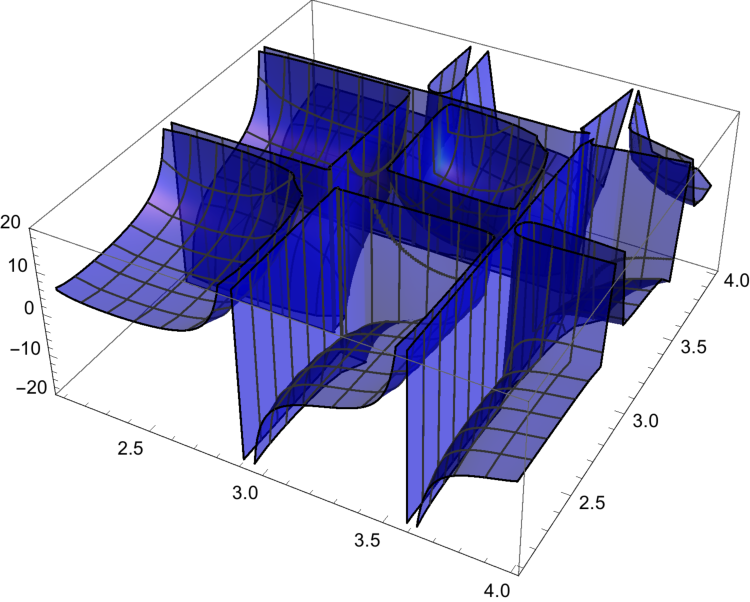
\includegraphics[width=0.4\textwidth]{figs/G3D} \hspace{30pt}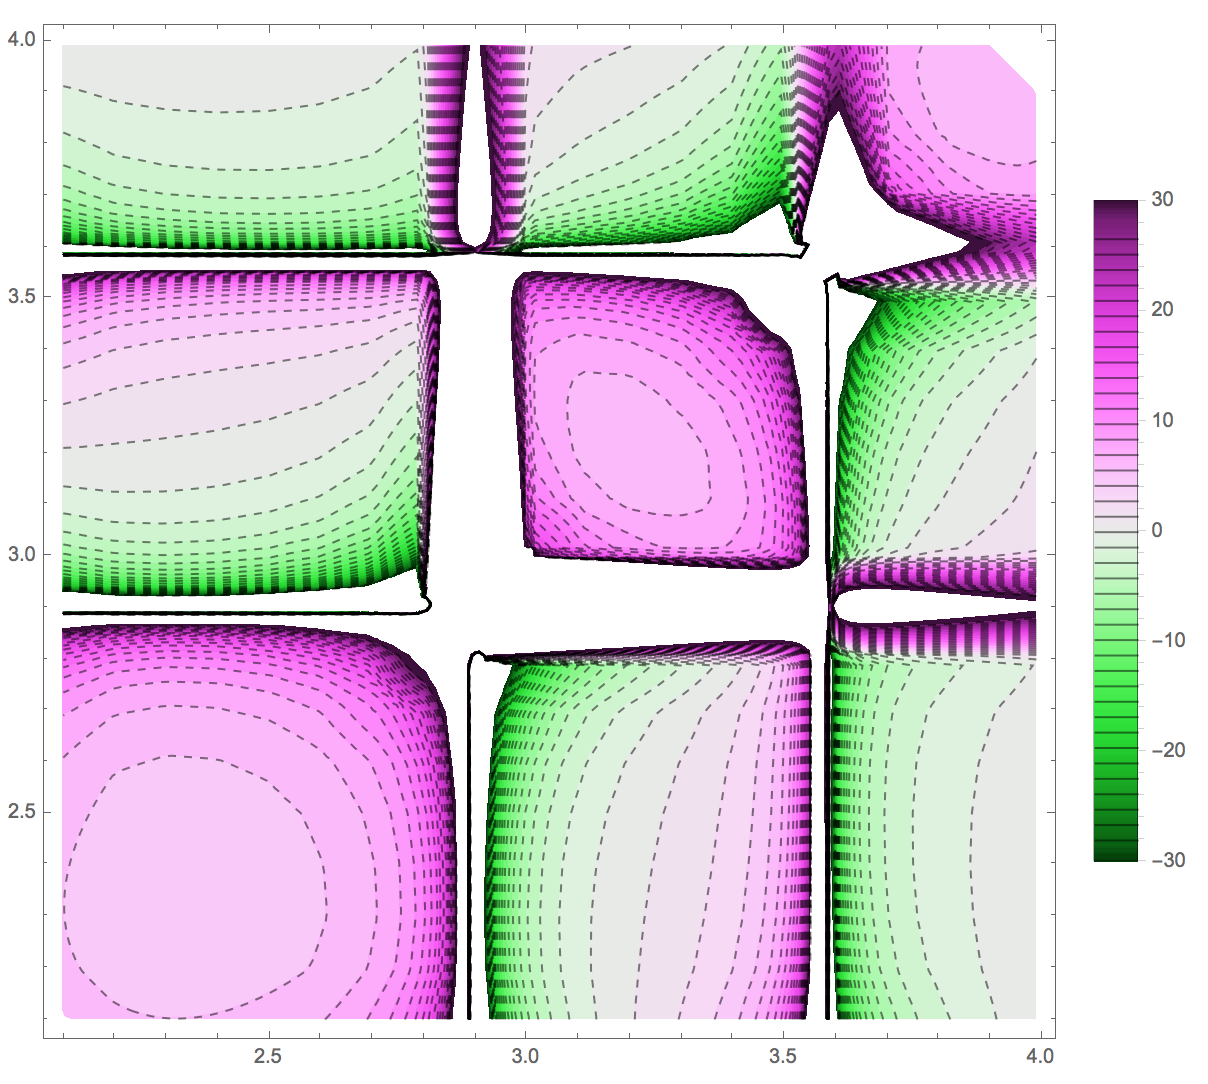
\includegraphics[width=0.35\textwidth]{figs/Gcontour}
\caption{$\mathcal G_{zz}(E_i,E_f,L)$ plotted as a function of $E_i, E_f$ in units of $M_\pi$, with $L$ fixed at $M_\pi L=6$. The singularities arise when either $E_i$ or $E_f$ (or both) coincide with one of the non-interacting two-pion energies. For interacting pions one must sample this function at the finite-volume energies (away from the poles) to determine $\mathcal G_{zz}$. Multiplying this with the pion vector form factor then gives the term needed to extract the $\textbf 2 + \mathcal J \to \textbf 2$ matrix element.
%
\label{fig:Gplot}}
\end{center}
\end{figure}




%\makeatletter
%\let\toc@pre\relax
%\let\toc@post\relax
%\makeatother 
%\listoffigures
%\listoftables

\clearpage
\bibliography{bibi}
\end{document}